%% =====================================================================
%%  B.Tech. Project Report -- Shreeyut Maheshwari (230003071), IIT Indore
%%  Build:  latexmk -pdf main.tex     (or: pdflatex, bibtex, pdflatex x2)
%% =====================================================================
\documentclass[12pt,a4paper,oneside]{report}

%% ---------------- Fonts, layout ----------------
\usepackage[T1]{fontenc}
\usepackage[utf8]{inputenc}
\usepackage{amsmath,amsthm}                % amsthm must precede newtxmath
\usepackage{newtxtext,newtxmath}            % Times-like, as in the Word template
\usepackage[a4paper,top=1in,bottom=1in,left=1.25in,right=1in]{geometry}
\usepackage{setspace}
\onehalfspacing
\usepackage{microtype}

%% ---------------- Mathematics ----------------
\usepackage{mathtools,bm}
\newtheorem{theorem}{Theorem}[chapter]
\newtheorem{lemma}[theorem]{Lemma}
\newtheorem{proposition}[theorem]{Proposition}
\newtheorem{corollary}[theorem]{Corollary}
\theoremstyle{definition}
\newtheorem{definition}[theorem]{Definition}
\theoremstyle{remark}
\newtheorem{remark}[theorem]{Remark}

%% ---------------- Figures, tables, algorithms ----------------
\usepackage{graphicx}
\graphicspath{{figures/}}
\usepackage{float}
\usepackage{booktabs,multirow,tabularx,array,makecell}
\usepackage{longtable}
\usepackage{caption,subcaption}
\captionsetup{font=small,labelfont=bf}
\usepackage{algorithm}
\usepackage[noend]{algpseudocode}
\usepackage{siunitx}
\sisetup{detect-all}
\usepackage{enumitem}
\setlist{itemsep=2pt,topsep=4pt}
\usepackage[dvipsnames,table]{xcolor}
\usepackage{listings}
\lstset{basicstyle=\ttfamily\scriptsize,breaklines=true,breakatwhitespace=false,frame=single,
        columns=fullflexible,keepspaces=true,showstringspaces=false,
        keywordstyle=\color{RoyalBlue}\bfseries,commentstyle=\color{ForestGreen},
        stringstyle=\color{BrickRed},numbers=left,numberstyle=\tiny\color{gray},
        language=Python}

%% ---------------- Headings, header/footer ----------------
\usepackage{titlesec}
\titleformat{\chapter}[display]
  {\normalfont\centering\bfseries}
  {\Large\chaptertitlename\ \thechapter}{8pt}{\LARGE}
\titlespacing*{\chapter}{0pt}{-10pt}{24pt}
\titleformat{\section}{\normalfont\large\bfseries}{\thesection}{0.8em}{}
\titleformat{\subsection}{\normalfont\normalsize\bfseries}{\thesubsection}{0.8em}{}

\usepackage{fancyhdr}
\pagestyle{fancy}
\fancyhf{}
\renewcommand{\headrulewidth}{0pt}
\fancyfoot[R]{\small Page \textbar\ \thepage}
\fancypagestyle{plain}{\fancyhf{}\renewcommand{\headrulewidth}{0pt}%
  \fancyfoot[R]{\small Page \textbar\ \thepage}}

%% ---------------- References, links ----------------
\usepackage[numbers,square,sort&compress]{natbib}
\usepackage{xurl}
\usepackage[hidelinks,bookmarksnumbered]{hyperref}
\usepackage[capitalise,nameinlink]{cleveref}

%% ---------------- Project macros ----------------
\newcommand{\ReSPect}{ReSPect}
\newcommand{\KalSea}{KalSea}
\newcommand{\NFE}{\mathrm{NFE}}
\newcommand{\Emb}{\mathrm{Emb}}
\newcommand{\Out}{\mathrm{Out}}
\newcommand{\SEA}{\mathrm{SEA}}
\newcommand{\Lone}{\mathrm{L1}_{\mathrm{rel}}}
\newcommand{\R}{\mathbb{R}}
\newcommand{\E}{\mathbb{E}}
\newcommand{\tr}{^{\top}}
%% Placeholder for metrics of the full-scale runs (to be filled in later)
\newcommand{\TBD}{\textcolor{BrickRed}{\textbf{[TBD]}}}

%% ---------------- Title information ----------------
\newcommand{\thesistitle}{Accelerating Diffusion Models with Training-Free Caching: ReSPect and KalSea, with Applications in Mechanical Engineering}
\newcommand{\thesistitleshort}{Accelerating Diffusion Models with Training-Free Caching}
\newcommand{\studentname}{Shreeyut Maheshwari}
\newcommand{\rollno}{230003071}
\newcommand{\guidename}{Dr.\ Mohd.\ Arshad}
\newcommand{\guidedesig}{Assistant Professor}
\newcommand{\guidedept}{Department of Mathematics}
\newcommand{\discipline}{Mechanical Engineering}
\newcommand{\submissiondate}{November 2026}

\hypersetup{pdftitle={\thesistitle},pdfauthor={\studentname}}

\begin{document}

%% =====================================================================
%%  FRONT MATTER
%% =====================================================================
\pagenumbering{arabic}

%% ---------------- Title page 1 ----------------
\clearpage\begingroup
\thispagestyle{plain}
\centering
\vspace*{0.4cm}
{\fontsize{26}{32}\selectfont\bfseries B. TECH. PROJECT REPORT\par}
\vspace{0.4cm}
{\fontsize{24}{30}\selectfont\bfseries On\par}
\vspace{0.4cm}
{\fontsize{21}{28}\selectfont\bfseries Accelerating Diffusion Models with\\ Training-Free Caching:\\ ReSPect and KalSea\par}
\vspace{0.3cm}
{\large\bfseries with Applications in Mechanical Engineering\par}
\vspace{1.2cm}
{\large BY\par}
\vspace{0.2cm}
{\large\bfseries \studentname\par}
{\large\bfseries \rollno\par}
\vspace{1.2cm}

\includegraphics[width=0.30\textwidth]{iiti_logo.jpg}\par
\vfill
{\large\bfseries DISCIPLINE OF MECHANICAL ENGINEERING\par}
{\large\bfseries INDIAN INSTITUTE OF TECHNOLOGY INDORE\par}
{\large\bfseries \submissiondate\par}
\par\endgroup\clearpage

%% ---------------- Title page 2 ----------------
\clearpage\begingroup
\thispagestyle{plain}
\centering
\vspace*{0.2cm}
{\fontsize{22}{29}\selectfont\bfseries Accelerating Diffusion Models with Training-Free Caching: ReSPect and KalSea, with Applications in Mechanical Engineering\par}
\vspace{1.0cm}
{\large\bfseries A PROJECT REPORT\par}
\vspace{0.6cm}
{\itshape Submitted in partial fulfillment of the\\ requirements for the award of the degree\par}
\vspace{0.6cm}
{\bfseries\itshape of\par}
{\large\bfseries BACHELOR OF TECHNOLOGY\par}
{\bfseries in\par}
\vspace{0.4cm}
{\large\bfseries MECHANICAL ENGINEERING\par}
\vspace{0.6cm}
{\itshape Submitted by:\par}
{\large\bfseries \studentname\par}
\vspace{0.5cm}
{\itshape Guided by:\par}
{\large\bfseries \guidename\par}
\vspace{0.6cm}

\includegraphics[width=0.28\textwidth]{iiti_logo.jpg}\par
\vfill
{\large\bfseries INDIAN INSTITUTE OF TECHNOLOGY INDORE\par}
{\large\bfseries \submissiondate\par}
\par\endgroup\clearpage

%% ---------------- Declaration and certificate ----------------
\chapter*{}
\vspace{-2.5cm}
\begin{center}
{\large\bfseries\underline{CANDIDATE'S DECLARATION}}
\end{center}
\vspace{0.4cm}
\noindent I hereby declare that the project entitled \textbf{``\thesistitle,''} submitted in partial fulfillment for the award of the degree of Bachelor of Technology in `\discipline' completed under the supervision of \textbf{\guidename, \guidedesig,} IIT Indore is an authentic work.

\medskip
Further, I declare that I have not submitted this work for the award of any other degree elsewhere.

\vspace{1.6cm}
\begin{flushright}
\rule{6cm}{0.4pt}\\
\textbf{Signature and name of the student with the date}\\
\studentname\ (\rollno)
\end{flushright}
\noindent\rule{\textwidth}{1pt}
\begin{center}
{\large\bfseries\underline{CERTIFICATE by BTP Guide}}
\end{center}
\vspace{0.3cm}
\noindent It is certified that the above statement made by the student is correct to the best of my knowledge.

\vspace{1.8cm}
\begin{flushright}
\rule{6cm}{0.4pt}\\
\textbf{Signature of BTP Guide with date and designation}\\
\textbf{\guidename}\\
\textbf{\guidedesig}\\
\textbf{\guidedept}\\
\textbf{IIT Indore}
\end{flushright}

%% ---------------- Preface ----------------
\chapter*{Preface}
\addcontentsline{toc}{chapter}{Preface}
This report on ``\thesistitle'' was prepared under the guidance of \guidename. It describes my B.Tech.\ project on making diffusion models, the generative models behind current image and video generators and an increasing number of engineering design tools, faster to sample without retraining them. The project started with a literature review of training-free feature caching, in particular SeaCache and Spectrum, and led to two methods of my own: \emph{ReSPect} (Residual Spectral Prediction), which forecasts the skipped transformer residuals with a Chebyshev--Taylor predictor behind a spectrally aligned gate, and \emph{KalSea} (Kalman-Corrected Spectral-Evolution-Aware Caching), which replaces the open-loop forecast by a Kalman filter and corrects every skipped gap with predictor-corrector gap smoothing.

The report explains the theory behind both methods, their implementation for several open-weight models, their evaluation, and how they carry over to diffusion models used in mechanical engineering, namely structural topology optimization and the reconstruction of flow fields governed by partial differential equations. I have tried, to the best of my abilities, to explain the content in a lucid manner and have added figures, tables and algorithms to make it more illustrative.

\vspace{1cm}
\noindent\studentname\\
B.Tech.\ IV Year\\
Discipline of \discipline\\
IIT Indore

%% ---------------- Acknowledgments ----------------
\chapter*{Acknowledgments}
\addcontentsline{toc}{chapter}{Acknowledgments}
I extend my sincere gratitude to \guidename\ for his unwavering support and invaluable guidance throughout the course of this project. His encouragement to pursue a research problem in depth, and his insistence on careful analysis and honest comparison, shaped both methods described in this report. Without his mentorship this work would not have been possible.

I thank my co-author Abhishek Varshney (IIT Indore) for the many discussions on the methods and experiments, and Monty Anderson and Caleb Case (Prodia), co-authors of the ReSPect and KalSea papers, for their collaboration. I am also grateful to the authors of SeaCache, Spectrum, FLUX, HunyuanVideo, Wan2.1, Optimize Any Topology and DiffusionPDE for releasing their code and model weights, on which all experiments in this report are built. This experience has been both enlightening and rewarding.

\vspace{1cm}
\noindent\studentname\\
B.Tech.\ IV Year\\
Discipline of \discipline\\
IIT Indore

%% ---------------- Abstract ----------------
\chapter*{Abstract}
\addcontentsline{toc}{chapter}{Abstract}
%% Abstract
Diffusion and flow-matching transformers generate high-quality images and videos and are increasingly used in engineering design, but sampling them requires tens to thousands of sequential evaluations of a large network. Training-free feature caching reduces this cost by skipping the network on some steps; every cache must decide \emph{when} to compute and \emph{what} to write on the skipped steps. This project develops two caches that improve both decisions.

\emph{ReSPect} (Residual Spectral Prediction) couples a spectrally aligned gate, derived from the linear minimum-mean-square-error (Wiener) denoiser, with a forecaster of the transformer \emph{residual} that blends a ridge-regularised Chebyshev fit of the residual history with a first-order discrete Taylor correction. We show that its forecast error admits a bound independent of the skip length, whereas the bounds of copy-reuse and Taylor extrapolation grow with it, and we derive the blend weight and warm-up analytically. ReSPect achieves speedups of $3.30\times$, $2.63\times$ and $2.77\times$ on FLUX.1-dev, Wan2.1-1.3B and HunyuanVideo with lower output error than existing caching baselines at matched or lower compute, improving PSNR by up to 3.46, 11.4 and 9.9\,dB.

\emph{KalSea} (Kalman-Corrected Spectral-Evolution-Aware Caching) observes that all existing fillers are open loop: the error made on skipped steps is integrated into the sample and never corrected. Behind the same gate, a damped-trend Kalman filter forecasts the residual, and \emph{predictor--corrector gap smoothing} (PCGS) uses the Rauch--Tung--Striebel smoother to correct every skipped gap once the next step is computed, re-integrating it through the output layers only, with no additional transformer evaluations. On FLUX.1-dev, KalSea reaches 27.72\,dB PSNR with respect to the 50-step sampler at 18.1 of 50 evaluations (SeaCache: 26.29\,dB at 18.4) and 22.53 vs.\ 21.33\,dB at 13 evaluations; PCGS alone contributes 0.81 and 0.61\,dB, and KalSea improves over SeaCache on HunyuanVideo and Wan2.1 by up to 3.2 and 2.3\,dB in the same setup.

Finally, we carry both caches over to two open-weight diffusion models from mechanical engineering, Optimize Any Topology for structural topology optimisation and DiffusionPDE for the reconstruction of a flow past a cylinder, by generalising the residual split to U-Net denoisers and the corrector to DDIM with classifier-free guidance and to gradient-guided second-order samplers. On DiffusionPDE's Navier--Stokes forward and inverse problems, KalSea needs $1.7$--$2.6\times$ fewer network evaluations than the 2000-step sampler, recovers the flow with 3.3\% error on the forward problem of the first released case, and is more accurate than ReSPect in all eight comparisons, showing that the closed loop is essential when guidance gradients are approximated on skipped steps.


%% ---------------- Lists ----------------
\cleardoublepage
\renewcommand{\contentsname}{Table of Contents}
\tableofcontents
\listoffigures
\addcontentsline{toc}{chapter}{List of Figures}
\listoftables
\addcontentsline{toc}{chapter}{List of Tables}
% List of abbreviations
\chapter*{List of Abbreviations}
\addcontentsline{toc}{chapter}{List of Abbreviations}
{\renewcommand{\arraystretch}{1.15}
\begin{longtable}{@{}ll@{}}
  \toprule
  Abbreviation & Meaning \\
  \midrule
  \endfirsthead
  \toprule
  Abbreviation & Meaning \\
  \midrule
  \endhead
  \bottomrule
  \endfoot
  adaLN & Adaptive layer normalisation \\
  CE & Compliance error \\
  CFG & Classifier-free guidance \\
  CI & Confidence interval \\
  DCT & Discrete cosine transform \\
  DDIM & Denoising diffusion implicit model \\
  DDPM & Denoising diffusion probabilistic model \\
  DiT & Diffusion transformer \\
  DPS & Diffusion posterior sampling \\
  EDM & Elucidated diffusion model (Karras et al.) \\
  FEA & Finite-element analysis \\
  FM & Flow matching \\
  IoU & Intersection over union \\
  KalSea & Kalman-corrected spectral-evolution-aware caching \\
  LDM & Latent diffusion model \\
  LMMSE & Linear minimum mean-square error \\
  LPIPS & Learned perceptual image patch similarity \\
  MAE & Mean absolute error \\
  NFAE & Neural-field autoencoder \\
  NFE & Number of (network) function evaluations \\
  OAT & Optimize Any Topology \\
  ODE & Ordinary differential equation \\
  PCGS & Predictor--corrector gap smoothing \\
  PDE & Partial differential equation \\
  PSNR & Peak signal-to-noise ratio \\
  ReSPect & Residual spectral prediction (for efficient caching of transformers) \\
  RTS & Rauch--Tung--Striebel (smoother) \\
  SEA & Spectral-evolution-aware (filter / gate) \\
  SIMP & Solid isotropic material with penalisation \\
  SNR & Signal-to-noise ratio \\
  SSIM & Structural similarity index \\
  TFLOPs & Tera floating-point operations \\
  UniPC & Unified predictor--corrector solver \\
  VAE & Variational autoencoder \\
  VFE & Volume-fraction error \\
  VP & Variance preserving \\
\end{longtable}}


%% =====================================================================
%%  MAIN MATTER
%% =====================================================================
\chapter{Introduction}\label{ch:introduction}

\section{Background and motivation}

Diffusion models \citep{sohl2015deep,ho2020ddpm,song2021sde} and their flow-matching counterparts \citep{lipman2023flow,liu2023rectifiedflow} are the dominant family of generative models today. They produce images and videos of remarkable quality, and they are increasingly used in science and engineering: to propose optimal structures in topology optimisation \citep{maze2023topodiff,nobari2025oat}, to design mechanical metamaterials \citep{bastek2023inverse} and CAD models \citep{xu2024brepgen}, and to reconstruct flow fields governed by partial differential equations \citep{shu2023physics,huang2024diffusionpde}. Their strength comes at a price. A diffusion model generates a sample by starting from random noise and removing it gradually: a numerical solver integrates a learned differential equation over tens to thousands of steps, and every step requires a full evaluation of a large neural network. In the current text-to-image and text-to-video models, this network is a diffusion transformer (DiT) \citep{peebles2023dit} with billions of parameters that processes thousands of tokens; FLUX.1-dev, for example, needs about five seconds on a state-of-the-art GPU for a single $1024\times1024$ image, and HunyuanVideo more than a minute for a short video clip.

Many approaches reduce this cost, from faster solvers to distillation into few-step students and quantisation (\cref{sec:lit-accel}). Most of them require additional training or change the model's outputs. \emph{Feature caching} is different: it exploits the observation that the network's internal activations change only slightly between consecutive steps. On some steps, the expensive part of the network is skipped and its output is approximated from the steps that were computed. Caching is training-free, leaves the weights and the sampler unchanged, and can be combined with the other approaches.

Every cache has to make two decisions at every step:
\begin{enumerate}
  \item \textbf{When to compute:} should the network be evaluated at this step, or can it be skipped?
  \item \textbf{What to write:} if the step is skipped, what should be written in place of the missing network output?
\end{enumerate}
The quality of a cache depends on both. A cache that skips at the wrong moments, for example when the content of the image is still forming, loses detail however good its approximation; a cache that skips at the right moments but writes a stale copy of an old output cannot skip many steps in a row.

\section{Problem statement}

At the start of this project, the most relevant prior methods each addressed one of the two decisions. SeaCache \citep{chung2026seacache} decides \emph{when} to compute with a gate that measures the change of the network input after a spectral filter derived from the optimal linear denoiser, so that the gate responds to the content rather than to the noise; but on skipped steps it simply reuses the last computed output. Spectrum \citep{han2026spectrum} decides \emph{what} to write by fitting the whole history of the network's features with Chebyshev polynomials; but it forecasts the full hidden state and is used with simple schedules. Moreover, every filler in the literature, whether it reuses or forecasts, is \emph{open loop}: when the next computed step reveals how wrong the filler was, its error has already been integrated into the sample and is never corrected. Finally, caching had been developed almost exclusively for text-to-image and text-to-video models, although engineering diffusion models are often sampled with even more steps.

This project therefore addresses the following questions:
\begin{itemize}
  \item How should a spectrally aligned gate be combined with a long-horizon forecaster, and what exactly should be forecast?
  \item Can the forecaster's design choices be derived rather than tuned, and what can be proven about its error as a function of the skip length?
  \item Can the observation made at each computed step be used to correct the steps that were skipped before it, without additional network evaluations?
  \item Do these techniques carry over to diffusion models used in mechanical engineering?
\end{itemize}

\section{Objectives and contributions}

The objectives of the project were to develop training-free caches that improve the quality--compute trade-off of diffusion transformers at matched compute, to justify their design theoretically, to evaluate them on large open image and video models, and to apply them to mechanical-engineering diffusion models. The contributions are:
\begin{enumerate}
  \item \textbf{ReSPect} (Residual Spectral Prediction, \cref{ch:respect}): a cache that couples the spectrally aligned gate with a forecaster of the transformer \emph{residual}, combining a ridge-regularised Chebyshev fit of the residual history with a first-order Taylor correction. We prove error bounds that rank copy-reuse, Taylor extrapolation and Chebyshev forecasting by their dependence on the skip length, show why residuals are better regression targets than hidden states, and derive the blend weight and warm-up analytically. ReSPect achieves speedups of $3.30\times$, $2.63\times$ and $2.77\times$ on FLUX.1-dev, Wan2.1 and HunyuanVideo with lower error than existing caches at matched or lower compute.
  \item \textbf{KalSea} (Kalman-Corrected Spectral-Evolution-Aware Caching, \cref{ch:kalsea}): a cache whose damped-trend Kalman forecaster is followed by \emph{predictor--corrector gap smoothing} (PCGS), which, once the next step is computed, smooths the residuals of the skipped gap with the Rauch--Tung--Striebel smoother, re-integrates the gap through the cheap output layers and continues from the corrected sample. PCGS needs no extra network evaluations and closes the loop that all previous caches leave open. On FLUX.1-dev KalSea reaches 27.72\,dB PSNR at 18.1 of 50 evaluations, compared with 26.29\,dB published for SeaCache, and it improves on SeaCache on both video models.
  \item \textbf{Open implementations} of both methods for FLUX.1-dev, HunyuanVideo and Wan2.1, and for KalSea additionally FLUX.2 [dev] and MiniMax-H3, verified against exact invariants.
  \item \textbf{Applications in mechanical engineering} (\cref{ch:applications}): a generalisation of both caches to U-Net denoisers, DDIM with classifier-free guidance and gradient-guided EDM samplers, and their evaluation on two recent open-weight models, Optimize Any Topology for structural topology optimisation (full OpenTO test split, evaluated with the model's own finite-element compliance analysis) and DiffusionPDE for flow-field reconstruction around a cylinder (forward and inverse Navier--Stokes problems), where KalSea reduces the network evaluations of the 2000-step guided sampler by $1.7$--$2.6\times$.
\end{enumerate}
The two methods are also described in two research papers that I co-authored with Abhishek Varshney, \guidename, Monty Anderson and Caleb Case.

\section{Organisation of the report}

\Cref{ch:literature} reviews diffusion models, acceleration methods, training-free caching, Kalman filtering and smoothing, and diffusion models in mechanical engineering, and identifies the research gaps. \Cref{ch:background} introduces the notation, the residual-caching formulation, the derivation of the spectrally aligned gate and the evaluation methodology. \Cref{ch:respect,ch:kalsea} present ReSPect and KalSea with their theory, implementation and experiments, and compare the two. \Cref{ch:applications} applies both methods to topology optimisation and flow-field reconstruction. \Cref{ch:conclusion} concludes and outlines future work. \Cref{app:code} reproduces the key parts of the code.

\chapter{Literature Review}\label{ch:literature}

This chapter reviews the work on which the project builds. \Cref{sec:lit-generative} summarises diffusion and flow-matching models and the transformer backbones that are accelerated in this report. \Cref{sec:lit-accel} places training-free caching among the other families of acceleration methods. \Cref{sec:lit-caching,sec:lit-seacache,sec:lit-forecast} review caching in detail, organised by the two decisions every cache makes: \emph{when} to evaluate the network and \emph{what} to write on the steps it skips. SeaCache and Spectrum, the two methods closest to this project, are discussed in depth. \Cref{sec:lit-filtering} covers the estimation theory (Kalman filtering and smoothing) on which KalSea rests, and \cref{sec:lit-mech} surveys diffusion models in mechanical engineering, the target of the applications in \cref{ch:applications}. The chapter closes with the research gaps that motivated ReSPect and KalSea (\cref{sec:lit-gaps}).

%% ------------------------------------------------------------------------------------------------
\section{Diffusion and flow-matching generative models}\label{sec:lit-generative}

\paragraph{Denoising diffusion.} Diffusion models were introduced by \citet{sohl2015deep} as a sequence of small Gaussian perturbations that gradually destroys the structure of the data, together with a learned reverse process that restores it. \citet{ho2020ddpm} made the approach practical with denoising diffusion probabilistic models (DDPM): a network is trained to predict the noise added to a clean sample at a randomly chosen noise level, and sampling runs the learned reverse chain over hundreds to a thousand steps. \citet{song2021sde} unified diffusion and score matching through stochastic differential equations and showed that every diffusion process has a deterministic \emph{probability-flow} ordinary differential equation (ODE) with the same marginals. Deterministic samplers integrate this ODE: DDIM \citep{song2021ddim} reduces the number of steps to tens, and the EDM framework of \citet{karras2022edm} separates the design choices of noise schedule, network preconditioning and solver (with a second-order Heun sampler). Improvements to the noise schedule, such as the cosine schedule of \citet{nichol2021improved} and the zero-terminal-SNR rescaling of \citet{lin2024zerosnr}, are used by several of the models in this report.

\paragraph{Latent diffusion and guidance.} Latent diffusion models \citep{rombach2022ldm} run the diffusion process in the compressed latent space of an autoencoder, which makes high-resolution generation affordable; all image and video models in this report, as well as the topology-optimisation model of \cref{ch:applications}, are latent models. Conditional generation is usually sharpened by classifier-free guidance \citep{ho2022cfg}, which combines a conditional and an unconditional network evaluation at every step and therefore doubles the sampling cost, or is distilled into a single guidance-conditioned evaluation, as in FLUX.1-dev.

\paragraph{Flow matching and rectified flow.} Flow matching \citep{lipman2023flow}, rectified flow \citep{liu2023rectifiedflow} and stochastic interpolants \citep{albergo2023stochastic} learn a velocity field that transports noise to data along (nearly) straight paths $x_\sigma = (1-\sigma)x_\star + \sigma\epsilon$. Sampling integrates the learned velocity with Euler steps over a decreasing schedule of $\sigma$. Scaled to large transformers \citep{esser2024sd3}, this formulation is the basis of the current open text-to-image and text-to-video models.

\paragraph{Diffusion transformers.} Early diffusion models used convolutional U-Nets \citep{ronneberger2015unet,dhariwal2021diffusion}. \citet{peebles2023dit} replaced the U-Net by a transformer \citep{vaswani2017attention} operating on a sequence of latent patches, with the timestep (and class) injected by adaptive layer normalisation (adaLN), and showed that quality improves steadily with model size. The models accelerated in this report are diffusion transformers (DiTs):
\begin{itemize}
  \item \textbf{FLUX.1-dev} \citep{bfl2024flux}, a rectified-flow text-to-image model with 19 double-stream blocks (separate image and text streams with joint attention) followed by 38 single-stream blocks, and guidance distilled into the network;
  \item \textbf{HunyuanVideo} \citep{kong2024hunyuanvideo}, a large text-to-video DiT with a similar dual-/single-stream design;
  \item \textbf{Wan2.1} \citep{wan2025wan}, a text-to-video DiT family (the 1.3B model is used here) sampled with classifier-free guidance and a multistep UniPC solver \citep{zhao2023unipc}.
\end{itemize}
Generating one image or video with these models requires tens of sequential evaluations of a network with billions of parameters over thousands of tokens, which is the cost that this project reduces.

%% ------------------------------------------------------------------------------------------------
\section{Approaches to faster sampling}\label{sec:lit-accel}

The cost of sampling is (number of network evaluations) $\times$ (cost per evaluation). Existing acceleration methods attack one or both factors.

\paragraph{Fast solvers.} Higher-order and multistep ODE solvers reduce the number of steps needed for a given accuracy: DDIM \citep{song2021ddim}, the Heun sampler of EDM \citep{karras2022edm}, DPM-Solver and DPM-Solver++ \citep{lu2022dpmsolver,lu2025dpmsolverpp}, and the predictor--corrector framework UniPC \citep{zhao2023unipc}. Below roughly ten to twenty steps, however, the truncation error of any solver becomes visible.

\paragraph{Distillation.} Progressive distillation \citep{salimans2022progressive}, consistency models \citep{song2023consistency}, latent consistency models \citep{luo2023lcm}, adversarial diffusion distillation \citep{sauer2024add} and distribution matching distillation \citep{yin2024dmd} train a student that samples in one to a few steps. They are very effective but require an expensive training run per model and change the model's outputs.

\paragraph{Quantisation and efficient architectures.} Post-training quantisation such as Q-Diffusion \citep{li2023qdiffusion} and ViDiT-Q \citep{zhao2024viditq} lowers the cost of each evaluation, as do efficient attention kernels.

\paragraph{Feature caching.} Caching exploits the strong similarity of the network's internal activations at consecutive sampling steps: on some steps, all or part of the network is skipped and its output is approximated from steps that were computed. Caching is \emph{training-free}, leaves the weights and the sampler unchanged, and is complementary to the approaches above. Every cache makes two coupled decisions \citep{chung2026seacache}:
\begin{enumerate}
  \item a \textbf{schedule} (or gate) decides \emph{when} the network is evaluated, and
  \item a \textbf{reconstructor} (or filler) decides \emph{what} is written to the features on the steps it skips.
\end{enumerate}
The two are coupled through the length of the skipped runs: a content-aware gate cannot preserve quality on long skips if the skipped features are a stale copy, and an accurate long-horizon predictor cannot be used aggressively if the gate responds to noise rather than to content.

%% ------------------------------------------------------------------------------------------------
\section{Training-free feature caching}\label{sec:lit-caching}

\subsection{Caching in U-Nets and diffusion transformers}
DeepCache \citep{ma2024deepcache} observed that the high-level features of a U-Net change slowly across steps and recomputed only the shallow branch on most steps; block caching \citep{wimbauer2024blockcache} reuses the outputs of individual blocks whose change is predicted to be small. For diffusion transformers, $\Delta$-DiT \citep{chen2024deltadit} caches the deviation of block outputs at the front or back of the network depending on the sampling stage, FORA \citep{selvaraju2024fora} reuses the attention and MLP outputs at a fixed interval, and ToCa \citep{zou2025toca} selects individual tokens to recompute. Video models add a temporal axis of redundancy: Pyramid Attention Broadcast (PAB) \citep{zhao2024pab} broadcasts attention outputs at different rates for spatial, temporal and cross attention, and FasterCache \citep{lv2025fastercache} reuses features and the guidance branch. Learning-to-Cache \citep{ma2024l2c} learns which layers to cache, and OmniCache \citep{chu2025omnicache} distributes reuse globally over the sampling trajectory and filters the noise that reuse introduces.

\subsection{Dynamic gates: deciding when to compute}
Fixed-interval caches spend computation uniformly, although the network output changes quickly at some stages of sampling and slowly at others. Dynamic gates decide online. AdaCache \citep{kahatapitiya2025adacache} adapts the caching schedule to each video using a motion-aware signal. TeaCache \citep{liu2025teacache} accumulates the relative $\ell_1$ change of the timestep-modulated input of the first transformer block, which is available before the expensive blocks run, and recomputes once the sum exceeds a threshold $\delta$; on skipped steps it adds the last computed \emph{residual} of the block stack. MagCache \citep{ma2025magcache} models the magnitude ratio of successive residuals, DiCache \citep{bu2025dicache} probes a shallow layer to estimate the change of the deep features, and FreqCa \citep{liu2025freqca} treats frequency bands differently. These gates use the raw change of a feature as the signal. As argued in the ReSPect paper, this raw distance is a noise-contaminated drift: at early steps the noise contribution can dominate it, so the gate reacts to stochastic variation rather than to the evolving content.

%% ------------------------------------------------------------------------------------------------
\section{SeaCache: a spectrally aligned gate}\label{sec:lit-seacache}

SeaCache \citep{chung2026seacache} keeps TeaCache's accumulate-and-reset rule but measures the change \emph{after} a spectral-evolution-aware (SEA) filter. Modelling the latent at step $t$ as $x_t = a_t x_0 + b_t\epsilon$ with white noise $\epsilon$, the linear minimum-mean-square-error estimator of $x_0$ from $x_t$ is a convolution whose frequency response is the Wiener filter
\begin{equation}
  G_t(f) = \frac{a_t S_x(f)}{a_t^2 S_x(f) + b_t^2},
\end{equation}
where $S_x$ is the power spectrum of clean latents. Under a power-law prior $S_x(f)\propto |f|^{-\beta}$, $G_t$ is a low-pass filter at early (noisy) steps and admits progressively higher frequencies as sampling proceeds, reproducing the well-known coarse-to-fine evolution of diffusion sampling. SeaCache filters the first block's modulated input with the gain-normalised $G_t$ for the current noise level and accumulates the relative $\ell_1$ change of the filtered input, so that the gate responds to content rather than noise. It uses $\beta=2$ for images and $\beta=3$ for videos, always computes the first and last steps, and on skipped steps \emph{reuses} the last computed residual. The full derivation is given in \cref{sec:bg-sea}.

During this project two observations about SeaCache became important. First, its reconstructor is plain reuse, whose error grows linearly with the skip length (\cref{ch:respect}); SeaCache improves \emph{when} to compute but not \emph{what} to write. Second, its released HunyuanVideo script binds the scheduler that exists when the model is loaded, whereas the HunyuanVideo sampler creates a fresh scheduler for sampling. The gate therefore reads a stale noise level close to one instead of the sampling schedule, which skips step 1 once $\delta\gtrsim 0.21$ and costs 12--14\,dB on the affected prompts. KalSea reads the live noise level of the sampler (\cref{ch:kalsea}).

%% ------------------------------------------------------------------------------------------------
\section{Forecasting and correcting skipped features}\label{sec:lit-forecast}

\subsection{From reuse to forecasting}
Reuse is a zero-order prediction. TaylorSeer \citep{liu2025taylorseer} replaces it by a Taylor extrapolation built from finite differences of the features cached at the most recent computed steps, which is accurate for short skips but uses only local information and amplifies noise at higher orders. HiCache \citep{feng2026hicache} replaces the Taylor basis by scaled Hermite polynomials. FoCa \citep{zheng2026foca} treats feature caching as an ODE and combines a second-order backward-differentiation predictor with a Heun-type calibration.

\subsection{Spectrum: global Chebyshev forecasting}
Spectrum \citep{han2026spectrum} forecasts the hidden-state trajectory globally. The solver index is mapped affinely to $\tau\in[-1,1]$, every feature channel is expanded in Chebyshev polynomials $T_0,\dots,T_M$ (\cref{fig:lit-chebyshev}), and the coefficients are fitted by ridge regression \citep{hoerl1970ridge} to all features recorded so far. The forecast at a skipped step evaluates the fitted expansion at its coordinate, and is blended with a first-order discrete Taylor step. Spectrum's analysis gives three results that ReSPect builds on: an order-$(P{+}1)$ remainder for an ideal degree-$P$ Taylor predictor, a truncation error of the Chebyshev expansion that decays as $\rho^{-M}$ for functions analytic in a Bernstein ellipse and is independent of the skip length \citep{trefethen2019approximation}, and a stability bound for the ridge estimator. Spectrum forecasts the full hidden state and is used with simple schedules.

\begin{figure}[t]
  \centering
  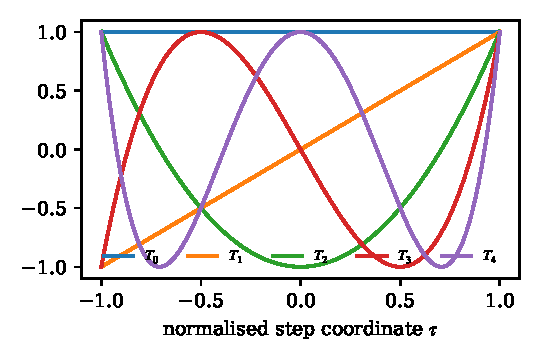
\includegraphics[width=0.55\textwidth]{lit_chebyshev.pdf}
  \caption[Chebyshev polynomials used by Spectrum and ReSPect]{The Chebyshev polynomials $T_0,\dots,T_4$ on the normalised step coordinate $\tau\in[-1,1]$. Spectrum and ReSPect fit each feature channel with a ridge-regularised expansion in this basis ($M=4$).}
  \label{fig:lit-chebyshev}
\end{figure}

\subsection{Correcting what is written}
Several recent methods check or repair the values written on skipped steps. SpeCa \citep{liu2025speca} accepts or rejects each forecast with a lightweight verification, OmniCache \citep{chu2025omnicache} filters the noise introduced by reused features, ERTACache \citep{peng2026ertacache} adjusts the integration intervals and rectifies cache-induced errors with a closed-form model profiled offline, and GP-Refiner \citep{shen2026gprefiner} regresses the deviation of forecast features online with a Gaussian process. Contemporaneous with KalSea, SpecKCast \citep{rajabi2026speckcast} tracks the DCT coefficients of the \emph{model output} with damped-trend Kalman filters along band-specific warped time and schedules computation by the filter's uncertainty. All of these methods improve the value used at the current or upcoming steps; none of them revises the latent of steps that have already been skipped. This observation is the starting point of KalSea (\cref{ch:kalsea}).

%% ------------------------------------------------------------------------------------------------
\section{Filtering, smoothing and predictor--corrector integration}\label{sec:lit-filtering}

The Kalman filter \citep{kalman1960} is the exact recursive minimum-mean-square-error estimator of the state of a linear-Gaussian state-space model; the Rauch--Tung--Striebel (RTS) smoother \citep{rauch1965rts} computes the estimates of past states given all observations, including later ones. Both are covered in the textbook of \citet{sarkka2013bayesian}. In target tracking, the integrated Wiener process (constant-velocity) model with state (position, velocity) is standard \citep{barshalom2001estimation}; damping the velocity, as in the damped-trend models of exponential smoothing \citep{gardner1985damped}, prevents forecasts over long horizons from overshooting, and the process-noise intensity can be adapted online so that the observed innovations match their predicted variance \citep{mehra1972adaptive}. Probabilistic ODE solvers \citep{schober2019probabilistic,tronarp2019probabilistic} infer the solution of an ODE from evaluations of its vector field by Gauss--Markov filtering and smoothing. In diffusion sampling, predictor--corrector schemes add Langevin steps \citep{song2021sde} or a second evaluation \citep{karras2022edm}, and UniPC \citep{zhao2023unipc} corrects a multistep solver by reusing the next network evaluation, which the sampler performs anyway. KalSea uses the RTS smoother for a different purpose: to infer the network evaluations that a cache \emph{skipped}.

%% ------------------------------------------------------------------------------------------------
\section{Diffusion models in mechanical engineering}\label{sec:lit-mech}

Deep generative models have become a design tool in mechanical engineering \citep{regenwetter2022deep}. Two application areas are relevant to this report.

\paragraph{Structural topology optimisation.} Topology optimisation distributes material in a design domain so as to minimise compliance (maximise stiffness) under loads, supports and a volume constraint. The homogenisation method of \citet{bendsoe1988generating} and density-based SIMP implementations such as the 99-line and 88-line codes \citep{sigmund2001,andreassen2011efficient} require a finite-element analysis at each of many iterations, which makes the optimisation expensive for large or repeated problems. Generative models learn to propose near-optimal structures directly. TopoDiff \citep{maze2023topodiff} showed that a conditional diffusion model guided by physical fields and surrogate models produces better structures than GAN-based approaches. \citet{giannone2023aligning} align the sampling trajectory of the diffusion model with the trajectory of the optimiser, and NITO \citep{nobari2024nito} uses neural implicit fields for resolution-free topology optimisation. Optimize Any Topology (OAT) \citep{nobari2025oat} combines a resolution- and shape-agnostic neural-field autoencoder with a conditional latent diffusion model trained on OpenTO, a dataset of 2.2 million optimised structures, and predicts minimum-compliance layouts for arbitrary aspect ratios, resolutions, volume fractions, loads and fixtures. Its denoiser is a conditional U-Net sampled with DDIM, and its code and weights are public, which makes it the first application in \cref{ch:applications}. Diffusion models are also used for other design tasks, such as boundary-representation CAD models \citep{xu2024brepgen} and mechanical metamaterials with a prescribed nonlinear response \citep{bastek2023inverse}.

\paragraph{Fluid mechanics and PDE-governed fields.} Physics-informed neural networks \citep{raissi2019pinn} and neural operators such as the Fourier neural operator \citep{li2021fno} learn solutions of partial differential equations (PDEs). Diffusion models add the ability to represent uncertainty and to reconstruct fields from incomplete data: \citet{shu2023physics} reconstruct high-fidelity flow fields from low-fidelity inputs with a physics-informed diffusion model, and \citet{kohl2023benchmarking} benchmark autoregressive conditional diffusion models for turbulent flow simulation. DiffusionPDE \citep{huang2024diffusionpde} learns the joint distribution of PDE coefficients (or initial states) and solutions with an EDM model and solves forward and inverse problems from sparse observations by guiding the sampler with the observation loss and the PDE residual, in the manner of diffusion posterior sampling \citep{chung2023dps}. Its sampler uses 2000 guided second-order steps, so sampling is the dominant cost, which makes it the second application in \cref{ch:applications}.

In both areas the generative model is evaluated many times per design or per solution, and design studies require many designs. Acceleration that is training-free and leaves the model unchanged is therefore directly useful, yet caching methods have so far been developed and evaluated almost exclusively on text-to-image and text-to-video models.

%% ------------------------------------------------------------------------------------------------
\section{Research gaps}\label{sec:lit-gaps}

\Cref{tab:lit-summary} summarises the caching methods along the two decisions of a cache. The review identifies the following gaps.
\begin{enumerate}
  \item \textbf{Gate and reconstructor are improved in isolation.} SeaCache improves the gate but keeps reuse; Spectrum improves the reconstructor but uses simple schedules. Since the two decisions are coupled through the skip length, neither can realise its benefit alone.
  \item \textbf{The regression target is larger than necessary.} Forecasting methods predict the full hidden state, although on a skipped step the block input is known exactly and only the block-stack residual is missing.
  \item \textbf{Hyper-parameters of forecasters are tuned empirically,} for example the blend between a local and a global predictor and the number of warm-up steps.
  \item \textbf{All fillers are open loop.} Reuse and every forecaster predict the skipped steps from the past only. When the next computed step reveals the error, the sampler has already integrated it into the latent, and no existing method revises the latent of the skipped steps.
  \item \textbf{Engineering diffusion models have not been accelerated by caching,} even though they are sampled with many steps and used in loops over many designs.
\end{enumerate}
ReSPect (\cref{ch:respect}) addresses gaps 1--3: it couples the SEA gate with a residual forecaster whose blend and warm-up are derived analytically. KalSea (\cref{ch:kalsea}) addresses gap 4 with predictor--corrector gap smoothing, and \cref{ch:applications} addresses gap 5.

\begin{table}[t]
  \centering
  \small
  \caption[Summary of training-free caching methods]{Training-free caching methods by their two decisions. ``Loop'': whether the error of the filler on skipped steps is corrected once the next computed step is observed.}
  \label{tab:lit-summary}
  \begin{tabularx}{\textwidth}{@{}l>{\raggedright\arraybackslash}X>{\raggedright\arraybackslash}Xl@{}}
    \toprule
    Method & When to compute (schedule) & What to write (filler) & Loop \\
    \midrule
    DeepCache, block caching & fixed / block-wise & reuse of U-Net features & open \\
    $\Delta$-DiT, FORA, ToCa, PAB & fixed interval, block / token level & reuse & open \\
    TeaCache, MagCache, DiCache & accumulated raw change & reuse of residual & open \\
    SeaCache & accumulated SEA-filtered change & reuse of residual & open \\
    TaylorSeer, HiCache & fixed interval & Taylor / Hermite extrapolation & open \\
    Spectrum & fixed / simple & Chebyshev ridge + Taylor (hidden state) & open \\
    FoCa & fixed interval & BDF2 predictor + Heun calibration & open \\
    SpecKCast & filter uncertainty & Kalman forecast of DCT output & open \\
    \midrule
    \textbf{ReSPect} (ours) & accumulated SEA-filtered change & Chebyshev ridge + Taylor (\emph{residual}), analytic blend & open \\
    \textbf{KalSea} (ours) & accumulated SEA-filtered change & Kalman forecast of residual + \emph{PCGS} & \textbf{closed} \\
    \bottomrule
  \end{tabularx}
\end{table}

\chapter{Background and Preliminaries}\label{ch:background}

This chapter fixes the notation used in the rest of the report. It describes how the models in this report are sampled (\cref{sec:bg-flow}), the anatomy of a diffusion transformer (\cref{sec:bg-dit}), the residual-caching formulation shared by ReSPect and KalSea (\cref{sec:bg-residual}), the spectrally aligned gate (\cref{sec:bg-sea}), and the metrics and protocol used to evaluate a cache (\cref{sec:bg-metrics}).

%% ------------------------------------------------------------------------------------------------
\section{Sampling diffusion and flow-matching models}\label{sec:bg-flow}

\paragraph{Flow matching.} Rectified-flow models \citep{lipman2023flow,liu2023rectifiedflow,albergo2023stochastic,esser2024sd3} interpolate linearly between a data sample $x_\star$ and Gaussian noise $\epsilon\sim\mathcal N(0,I)$,
\begin{equation}
  x_\sigma = (1-\sigma)\,x_\star + \sigma\,\epsilon, \qquad \sigma\in[0,1],
\end{equation}
and train a network $v_\theta(x_\sigma,\sigma,c)$ to predict the velocity $\epsilon - x_\star$ for a condition $c$ (e.g.\ a text prompt). Sampling starts from pure noise and integrates the learned velocity over a decreasing schedule $\sigma_0>\sigma_1>\dots>\sigma_N=0$ with Euler steps,
\begin{equation}\label{eq:bg-euler}
  x_{i+1} = x_i + (\sigma_{i+1}-\sigma_i)\, v_i, \qquad v_i = v_\theta(x_i,\sigma_i,c), \qquad i=0,\dots,N-1 .
\end{equation}
FLUX.1-dev uses this sampler with $N=50$ and a resolution-dependent shift of the schedule. Each step costs one evaluation of the network, so a sample costs $N$ network function evaluations (NFE).

\paragraph{Variance-preserving diffusion and DDIM.} DDPM-type models \citep{ho2020ddpm} define $x_t = \sqrt{\bar\alpha_t}\,x_0 + \sqrt{1-\bar\alpha_t}\,\epsilon$ for a decreasing signal level $\bar\alpha_t$. With the network predicting $\hat\epsilon$, $\hat x_0$, or the ``velocity'' $v = \sqrt{\bar\alpha_t}\epsilon - \sqrt{1-\bar\alpha_t}x_0$ \citep{salimans2022progressive}, the deterministic DDIM update \citep{song2021ddim} from $t$ to the previous timestep $t'$ is
\begin{equation}\label{eq:bg-ddim}
  x_{t'} = \sqrt{\bar\alpha_{t'}}\,\hat x_0 + \sqrt{1-\bar\alpha_{t'}}\,\hat\epsilon ,
\end{equation}
which, for every one of these parametrisations, is an \emph{affine} function of the network output: $x_{t'} = A_t x_t + B_t\, v_\theta(x_t,t)$. This linearity is all that KalSea's corrector needs (\cref{ch:kalsea}). Multistep solvers such as UniPC \citep{zhao2023unipc} combine several past outputs, but remain linear in the outputs for a fixed solver state.

\paragraph{Signal and noise coefficients.} Both families can be written as $x_t = a_t x_0 + b_t\epsilon$, with $(a_t,b_t)=(1-\sigma,\sigma)$ for flow matching and $(\sqrt{\bar\alpha_t},\sqrt{1-\bar\alpha_t})$ for variance-preserving diffusion. These coefficients are read from the sampler and determine the spectral filter of the gate (\cref{sec:bg-sea}).

%% ------------------------------------------------------------------------------------------------
\section{Anatomy of a diffusion transformer}\label{sec:bg-dit}

A diffusion transformer \citep{peebles2023dit} computes the network output in three stages:
\begin{equation}\label{eq:bg-stages}
  h^{\mathrm{in}}_i = \Emb(x_i), \qquad h^{\mathrm{out}}_i = F\big(h^{\mathrm{in}}_i, c_i\big), \qquad v_i = \Out\big(h^{\mathrm{out}}_i, c_i\big),
\end{equation}
where $\Emb$ embeds the latent patches into tokens, $F$ is the stack of transformer blocks, $\Out$ is a final adaptive normalisation followed by a linear projection back to latent patches, and $c_i$ embeds the timestep (and, for FLUX.1-dev, the guidance scale and pooled text). Each block modulates its inputs with adaptive layer normalisation:
\begin{equation}\label{eq:bg-adaln}
  \mathrm{AdaLN}(h, c) = \big(1+\gamma(c)\big)\odot\mathrm{LayerNorm}(h) + \beta(c),
\end{equation}
with scale $\gamma$ and shift $\beta$ regressed from $c$. In FLUX.1-dev, $F$ consists of 19 double-stream blocks, which keep separate image and text streams that interact through joint attention, followed by 38 single-stream blocks over the concatenated sequence; a $1024\times1024$ image corresponds to $64\times 64 = 4096$ image tokens. Almost all of the computation is in $F$; $\Emb$ and $\Out$ together cost a fraction of a percent of one evaluation. This asymmetry is what makes residual caching, and KalSea's corrector, cheap.

%% ------------------------------------------------------------------------------------------------
\section{Residual caching}\label{sec:bg-residual}

A residual cache stores the block-stack residual of the image tokens on computed steps,
\begin{equation}\label{eq:bg-residual}
  r_i = h^{\mathrm{out}}_i - h^{\mathrm{in}}_i ,
\end{equation}
and on skipped steps runs only $\Emb$ and $\Out$:
\begin{equation}\label{eq:bg-skip}
  \hat h^{\mathrm{out}}_j = h^{\mathrm{in}}_j + \hat r_j, \qquad \hat v_j = \Out\big(\hat h^{\mathrm{out}}_j, c_j\big),
\end{equation}
where the \emph{filler} $\hat r_j$ is the last computed residual (reuse, as in TeaCache and SeaCache) or a forecast (ReSPect, KalSea). Because $h^{\mathrm{in}}_j$ is computed exactly from the current latent, the reconstruction error of the block-stack output equals the error of the filler:
\begin{equation}\label{eq:bg-error}
  \hat h^{\mathrm{out}}_j - h^{\mathrm{out}}_j = \hat r_j - r_j .
\end{equation}
\Cref{fig:bg-residual} illustrates one computed and one skipped step. Note that the sampler still advances the latent on skipped steps (\cref{eq:bg-euler}) with the approximate velocity $\hat v_j$; any error of the filler is therefore integrated into the latent. This point is central to KalSea.

\begin{figure}[t]
  \centering
  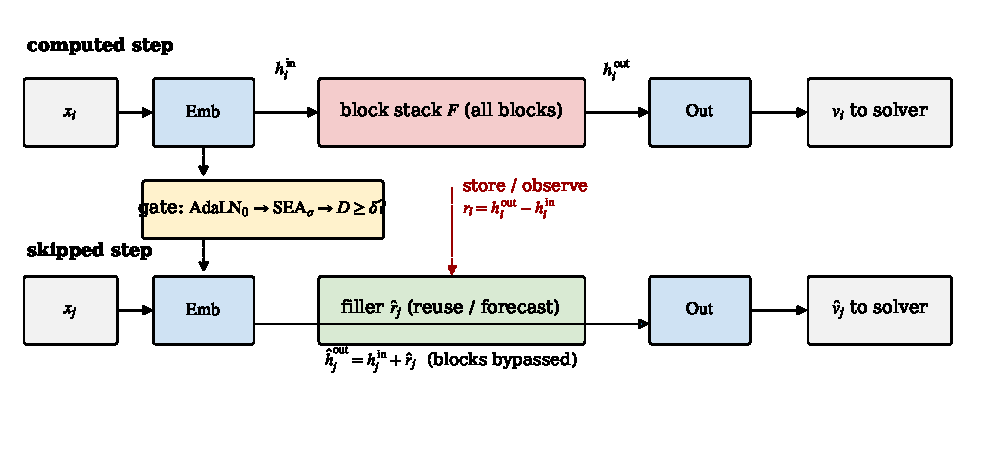
\includegraphics[width=0.92\textwidth]{bg_residual_cache.pdf}
  \caption[Residual caching]{Residual caching. On a computed step the full block stack $F$ runs and its residual $r_i = h^{\mathrm{out}}_i - h^{\mathrm{in}}_i$ is stored or observed. On a skipped step the blocks are bypassed: the filler $\hat r_j$ is added to the exactly computed input $h^{\mathrm{in}}_j$ and the result goes through the output layers. The gate decides which of the two paths a step takes.}
  \label{fig:bg-residual}
\end{figure}

%% ------------------------------------------------------------------------------------------------
\section{The spectrally aligned (SEA) gate}\label{sec:bg-sea}

\subsection{Gate input}
A gate must be evaluated at every step and must therefore be cheap. Following TeaCache \citep{liu2025teacache} and SeaCache \citep{chung2026seacache}, the gate reads the timestep-modulated input of the first block,
\begin{equation}
  I_i = \mathrm{AdaLN}_0\big(h^{\mathrm{in}}_i, c_i\big),
\end{equation}
which is available before any block runs and reflects both the latent and the noise level.

\subsection{Derivation of the Wiener response}
Model the latent at step $t$ as the linear mixture
\begin{equation}
  x_t = a_t x_0 + b_t \epsilon, \qquad \epsilon\sim\mathcal N(0,I),
\end{equation}
with $\epsilon$ white and independent of the clean latent $x_0$. This is a signal/noise model for the gate, not a claim about the exact forward process of each model. Consider the linear-MMSE estimator of $x_0$ from $x_t$, $h_t^\star = \arg\min_h \E\|h * x_t - x_0\|_2^2$. Assuming wide-sense stationarity, convolution is diagonal in the Fourier basis, and by Parseval's identity the risk of a filter with frequency response $H_t(f)$ splits per frequency:
\begin{equation}
  J_t(H_t) = \sum_f \Big[ |H_t(f)|^2\big(a_t^2S_x(f)+b_t^2\big) - 2\,\mathrm{Re}\big(H_t(f)\big)\,a_tS_x(f) + S_x(f)\Big],
\end{equation}
where $S_x$ is the power spectrum of $x_0$. Each summand is a scalar quadratic in $H_t(f)$; setting its derivative to zero gives $H_t(f)\big(a_t^2S_x(f)+b_t^2\big) = a_tS_x(f)$, i.e.\ the Wiener response \citep{wiener1949extrapolation}
\begin{equation}\label{eq:bg-wiener}
  G_t(f) = \frac{a_t\, S_x(f)}{a_t^2\, S_x(f) + b_t^2},
\end{equation}
which is a minimum because the second derivative $a_t^2S_x(f)+b_t^2$ is positive.

\paragraph{Spectral evolution.} Natural images follow a power law $S_x(f)\propto |f|^{-\beta}$ with $\beta\approx 2$. Inserting this prior into \cref{eq:bg-wiener}: at early steps ($a_t$ small) the denominator is dominated by the noise except near $f=0$, so $G_t$ is low-pass; as $a_t\to 1$ the passband widens towards high frequencies (\cref{fig:bg-wiener}a). This reproduces the coarse-to-fine evolution of diffusion sampling, in which global structure forms first and details later. SeaCache uses $\beta=2$ for images and $\beta=3$ for videos; for multi-dimensional token grids the filter is separable over the spatial (and temporal) axes.

\paragraph{Gain normalisation.} The raw responses differ by orders of magnitude in overall gain across steps, which would let high-gain steps dominate the accumulated distance. Each response is therefore normalised to unit mean gain over the frequency bins,
\begin{equation}\label{eq:bg-norm}
  G^{\mathrm{norm}}_t(f) = \nu_t\, G_t(f), \qquad \nu_t^{-1} = \frac{1}{L}\sum_{\ell} G_t(f_\ell),
\end{equation}
so that the accumulated distance measures changes of spectral shape rather than changes of filter gain (\cref{fig:bg-wiener}b).

\begin{figure}[t]
  \centering
  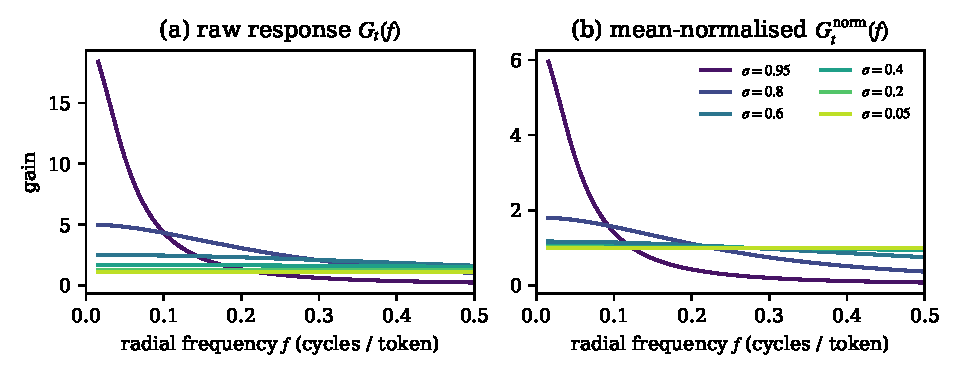
\includegraphics[width=0.95\textwidth]{bg_wiener.pdf}
  \caption[Wiener responses of the SEA filter]{Wiener responses of the SEA filter along a flow schedule ($a_t=1-\sigma$, $b_t=\sigma$, $S_x(f)=|f|^{-2}$), computed from the closed form of \cref{eq:bg-wiener}. (a) The raw response is low-pass at high noise and widens as $\sigma\to 0$. (b) After the mean-gain normalisation of \cref{eq:bg-norm}, the responses share a common scale and differ only in shape.}
  \label{fig:bg-wiener}
\end{figure}

\subsection{Accumulate-and-reset rule}
Let $\SEA_i(I) = \mathcal F^{-1}\big[G^{\mathrm{norm}}_{t_i}\odot\mathcal F(I)\big]$ denote the filtered gate input of step $i$ on its token grid. The gate computes the relative $\ell_1$ change between consecutive filtered inputs and accumulates it:
\begin{equation}\label{eq:bg-gate}
  d_i = \frac{\big\|\SEA_i(I_i) - \SEA_{i-1}(I_{i-1})\big\|_1}{\big\|\SEA_{i-1}(I_{i-1})\big\|_1}, \qquad D_i = D_{i-1} + d_i .
\end{equation}
Step $i$ is computed if $D_i\ge\delta$, after which $D_i$ is reset to zero, or if it is the first or the last step; otherwise it is skipped. The reference $\SEA_{i-1}(I_{i-1})$ is refreshed at \emph{every} step, computed or skipped, so that each $d_i$ measures only the incremental drift between consecutive solver states. The single threshold $\delta$ sets the compute budget: a larger $\delta$ skips more steps. Because the gate reads only the first block's modulated input, replacing the filler (reuse, ReSPect, KalSea) does not change where the gate fires, which allows fillers to be compared at an identical schedule.

%% ------------------------------------------------------------------------------------------------
\section{Evaluation methodology}\label{sec:bg-metrics}

\paragraph{Compute.} The compute of a cache is reported as the mean number of full block-stack evaluations per sample (NFE, out of 50 for the 50-step samplers), counted by hooks on the blocks. TFLOPs follow SeaCache's convention, and latency is the wall-clock time per sample on a single NVIDIA B200 GPU in bf16. Because a content-aware gate need not realise the same skip rate as another method at a shared $\delta$, methods are compared at \emph{matched or lower} compute, never at matched $\delta$.

\paragraph{Fidelity.} The goal of a cache is to reproduce the output of the uncached sampler. Every accelerated sample is therefore compared with the output of the uncached 50-step sampler for the same prompt and seed, using
\begin{itemize}
  \item \textbf{PSNR} on 8-bit RGB, $10\log_{10}(255^2/\mathrm{MSE})$ (higher is better);
  \item \textbf{SSIM} \citep{wang2004ssim}, the structural similarity index (higher is better);
  \item \textbf{LPIPS} \citep{zhang2018lpips}, a learned perceptual distance on AlexNet features (lower is better).
\end{itemize}
For videos the metrics are averaged over frames. In the KalSea study, differences between methods run in the same setup are reported with paired bootstrap 95\% confidence intervals over prompts (10{,}000 resamples, percentile method) and the fraction of prompts on which a method is better.

\paragraph{Benchmarks and models.} Text-to-image experiments use FLUX.1-dev \citep{bfl2024flux} at $1024\times1024$ with 50 steps, embedded guidance 3.5 and the 200 DrawBench prompts \citep{saharia2022imagen}, with the prompt index as seed. Text-to-video experiments use HunyuanVideo \citep{kong2024hunyuanvideo} and Wan2.1-T2V-1.3B \citep{wan2025wan} with 65 frames and 50 steps on VBench prompts \citep{huang2024vbench}. The exact settings of each study are given in \cref{ch:respect,ch:kalsea}.

\chapter{ReSPect: Residual Spectral Prediction}\label{ch:respect}

This chapter presents ReSPect (Residual Spectral Prediction for Efficient Caching of Transformers), the first method developed in this project. ReSPect is a training-free cache for diffusion transformers that combines the spectrally aligned gate of \cref{sec:bg-sea} with a forecaster of the skipped \emph{residuals}. The forecaster is a weighted sum of a ridge-regularised Chebyshev regression over the accumulated residual history, which captures the global trajectory, and a first-order discrete Taylor correction, which captures local dynamics. We show that its forecast error admits a skip-length-independent bound, whereas the bounds of copy-reuse and Taylor extrapolation grow with the skip length, and we derive its blend weight and warm-up length analytically. On FLUX.1-dev, Wan2.1-1.3B and HunyuanVideo, ReSPect achieves speedups of $3.30\times$, $2.63\times$ and $2.77\times$ over full evaluation with lower output error than existing caching baselines at matched or lower compute. The chapter follows our ReSPect paper, with the derivations given in full and an additional description of the implementation.

\begin{figure}[t]
  \centering
  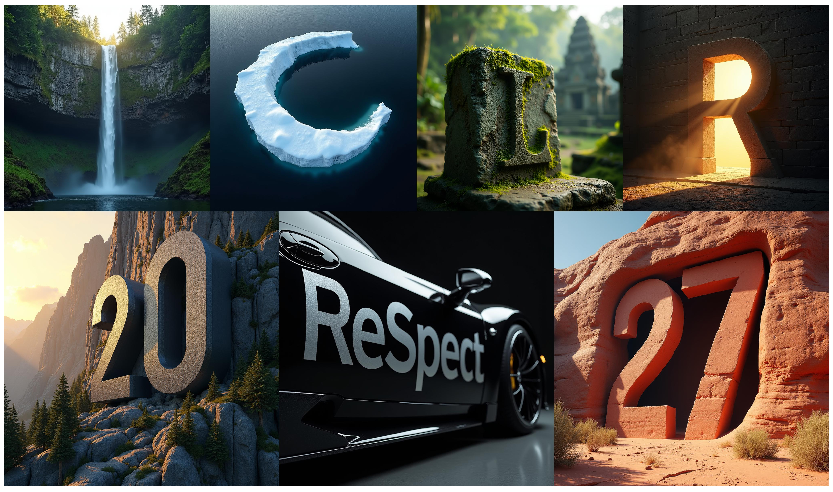
\includegraphics[width=0.95\textwidth]{respect_teaser.pdf}
  \caption[Images generated with ReSPect on FLUX.1-dev]{Images generated by FLUX.1-dev with ReSPect, which keeps high image fidelity at a $2.43\times$ acceleration.}
  \label{fig:respect-teaser}
\end{figure}

%% ------------------------------------------------------------------------------------------------
\section{Motivation}\label{sec:respect-motivation}

As discussed in \cref{sec:lit-accel}, a cache makes two coupled decisions at every step: a schedule decides whether the network is evaluated, and a reconstructor decides what is written to the features when it is not. Improving either one in isolation leaves the other as the bottleneck. The literature review identified two limitations:
\begin{itemize}
  \item \textbf{Noisy schedules.} Many gates use the raw distance between consecutive features \citep{liu2025teacache,bu2025dicache}. Under the mixture $x_t=a_tx_0+b_t\epsilon$ the noise contribution can dominate this distance at early steps, so the gate responds to stochastic variation. A timestep-dependent spectral filter isolates the content-sensitive drift (\cref{sec:bg-sea}).
  \item \textbf{Local reconstructors.} Most reconstructors use local temporal information, copying the last computed features \citep{selvaraju2024fora,zhao2024pab} or extrapolating from finite differences \citep{liu2025taylorseer}. Their approximation error grows with the skip length, and sample quality degrades at high speedups. Global trajectory fitting \citep{han2026spectrum} still predicts the full hidden state.
\end{itemize}
ReSPect specifies both decisions together (\cref{fig:respect-overview}). It keeps the spectrally aligned gate and forecasts only the transformer residual, because the block input at skipped steps is known exactly. This removes the predictable component from the regression target and yields a smaller, centred trajectory.

\begin{figure}[t]
  \centering
  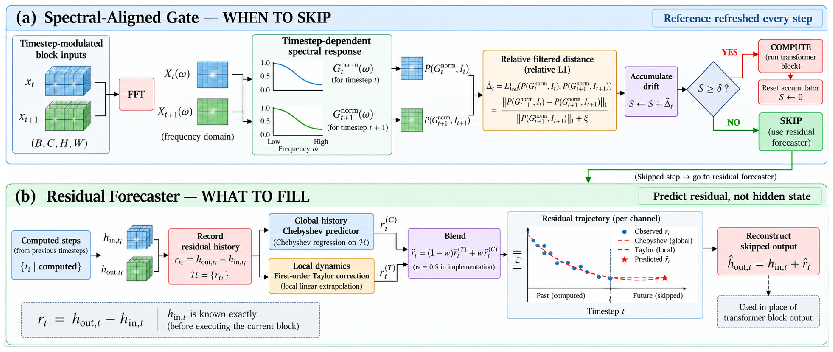
\includegraphics[width=\textwidth]{respect_overview.pdf}
  \caption[Overview of ReSPect]{Overview of ReSPect. (a) The spectrally aligned gate decides adaptively when to evaluate the network. (b) The residual forecaster combines a global Chebyshev prediction with a local first-order Taylor correction and writes $h^{\mathrm{in}}+\hat r$ on skipped steps.}
  \label{fig:respect-overview}
\end{figure}

%% ------------------------------------------------------------------------------------------------
\section{Problem setup}\label{sec:respect-setup}

Consider a latent generative model whose sampling trajectory $\{x_t\}_{t=0}^T$ is produced by a discrete solver, where $t\in\{0,\dots,T\}$ indexes solver steps from the initial noise towards the clean output. At step $t$ the latent $x_t$ is mapped to the input $I_t=\phi(x_t,t)$ of a transformer block, whose output $h^{\mathrm{out}}(t)$ is produced from the input $h^{\mathrm{in}}(t)$. The block residual
\begin{equation}\label{eq:respect-residual}
  r(t) = h^{\mathrm{out}}(t) - h^{\mathrm{in}}(t)
\end{equation}
induces a second trajectory $\{r(t)\}$ alongside $\{x_t\}$. On an evaluated step $h^{\mathrm{out}}(t)=h^{\mathrm{in}}(t)+r(t)$ holds by definition. On a skipped step the input is known and the reconstructor supplies $\hat r(t)$, yielding $\hat h^{\mathrm{out}}(t) = h^{\mathrm{in}}(t)+\hat r(t)$, so that the reconstruction error coincides with the residual error,
\begin{equation}\label{eq:respect-errid}
  \hat h^{\mathrm{out}}(t) - h^{\mathrm{out}}(t) = \hat r(t) - r(t)
\end{equation}
(\cref{eq:bg-error}). The reconstruction problem is therefore reduced to forecasting the residual trajectory at unevaluated steps.

\paragraph{The gate.} ReSPect uses the spectrally aligned gate of \cref{sec:bg-sea} unchanged in form: the first-block input is filtered with the gain-normalised Wiener response $G^{\mathrm{norm}}_t$ of \cref{eq:bg-wiener,eq:bg-norm}, each adjacent pair $(I_t,I_{t+1})$ is compared with its own pair of responses,
\begin{equation}
  \tilde\Delta_t = \Lone\big(\mathcal P(G^{\mathrm{norm}}_t,I_t),\,\mathcal P(G^{\mathrm{norm}}_{t+1},I_{t+1})\big), \qquad \mathcal P(G,I) = \mathcal F^{-1}\big[G\odot\mathcal F(I)\big],
\end{equation}
and the network is evaluated when the accumulated $\tilde\Delta_t$ exceeds $\delta$. The reference is refreshed at every step, including skipped steps, so each $\tilde\Delta_t$ measures only the incremental drift; on HunyuanVideo this choice is worth $+2.50$\,dB at matched compute (\cref{sec:respect-ablations}). The rest of this chapter specifies what is written on the skipped steps.

%% ------------------------------------------------------------------------------------------------
\section{Predictors on the sampling trajectory}\label{sec:respect-hierarchy}

We state the analysis for one residual channel; the predictor is applied independently across channels. Consider a skip from the last evaluated step $t_k$ to the current step $t_j$. Every reconstructor is a predictor $\hat r(t_j)$ built from the residuals recorded at evaluated steps; the candidates differ in the smoothness they assume of $r$.

\subsection{Order zero: copy-reuse}
Copy-reuse sets $\hat r(t_j)=r(t_k)$. If $r$ is $L$-Lipschitz on the sampling interval, then directly from the definition
\begin{equation}\label{eq:respect-reuse}
  |r(t_j)-r(t_k)| \le L\,|t_j-t_k| .
\end{equation}
The bound is tight, since $r(t)=Lt$ attains equality for every skip, and Lipschitz continuity is necessary in the worst case: for a non-Lipschitz residual the ratio $|r(t_j)-r(t_k)|/|t_j-t_k|$ is unbounded as the skip shrinks. Copy-reuse uses no derivative information, so additional smoothness ($r\in C^P$, $P\ge 1$) cannot improve the worst-case rate. \emph{The error of reuse grows linearly with the skip length.}

\subsection{Order $P$: Taylor extrapolation}
Assume $r\in C^{P+1}$. The degree-$P$ Taylor expansion of $r$ about $t_k$ is
\begin{equation}
  r(t_j) = \sum_{p=0}^{P}\frac{r^{(p)}(t_k)}{p!}(t_j-t_k)^p + R_P(t_j), \qquad R_P(t_j) = \frac{r^{(P+1)}(\xi)}{(P+1)!}(t_j-t_k)^{P+1}
\end{equation}
for some $\xi$ between $t_k$ and $t_j$. Hence $|R_P(t_j)|\le \|r^{(P+1)}\|_\infty |t_j-t_k|^{P+1}/(P+1)!$, an order-$(P{+}1)$ dependence on the skip length \citep[Thm.~3.1]{han2026spectrum}. This is the \emph{ideal} predictor, because it uses the exact derivatives at $t_k$, which a training-free cache never computes.

\paragraph{The implemented (discrete) predictor.} In practice the derivatives are replaced by backward differences formed from $P{+}1$ neighbouring evaluated residuals $s_0=t_k,s_1,\dots,s_P$, so the predictor is the degree-$P$ interpolant $p_P$ through those nodes, with remainder
\begin{equation}\label{eq:respect-interp}
  r(t_j)-p_P(t_j) = \frac{r^{(P+1)}(\xi)}{(P+1)!}\prod_{q=0}^{P}(t_j-s_q)
\end{equation}
for some $\xi$ in the convex hull of $\{t_j,s_0,\dots,s_P\}$. Only the $q=0$ factor shrinks with the skip length $\ell=|t_j-t_k|$; the remaining factors are fixed by the positions of the earlier evaluated nodes. The $(P{+}1)$-order rate therefore requires a node-spacing condition $\max_q|t_j-s_q|\le C_{\mathrm{node}}\,\ell$, under which $|r(t_j)-p_P(t_j)|\le C_{\mathrm{node}}^{P+1}\|r^{(P+1)}\|_\infty\,\ell^{P+1}/(P+1)!$. A dynamic gate does not guarantee a uniform $C_{\mathrm{node}}$: with the earlier nodes held fixed and $\ell\to 0$, the error is $O(\ell)$, not $O(\ell^{P+1})$.

\begin{proposition}[The failure is sharp]\label{prop:respect-sharp}
Take $P=1$, $r(t)=t^2$, nodes $s_0=t_k=0$ and $s_1=-H$ with $H>0$, and forecast point $t_j=\ell>0$. Then $|r(\ell)-p_1(\ell)|/\ell^2 = 1 + H/\ell$, which is unbounded as $H/\ell\to\infty$.
\end{proposition}
\begin{proof}
The linear interpolant through $(0,0)$ and $(-H,H^2)$ is $p_1(t)=-Ht$, so $|r(\ell)-p_1(\ell)| = \ell^2+H\ell = \ell(\ell+H)$. Dividing by $\ell^2$ gives the claim.
\end{proof}

Even uniform backward spacing does not recover the ideal rate: for $t_j=t_k+\ell$ and $s_q=t_k-qh$, $\prod_{q=0}^P|t_j-s_q|=\prod_{q=0}^P(\ell+qh)$ is a degree-$(P{+}1)$ polynomial in $\ell$ that coincides with $\ell^{P+1}$ only in the limit $h/\ell\to 0$. In addition, the difference operator amplifies observation noise by binomial coefficients of order $2^P$. A higher order therefore tightens the bound only for short skips and becomes unstable as $|t_j-t_k|$ grows, and the predictor discards all but the $P{+}1$ most recent evaluations. These bounds motivate a \emph{global} predictor that exploits the full observed trajectory.

%% ------------------------------------------------------------------------------------------------
\section{Residual forecasting with Chebyshev bases}\label{sec:respect-cheb}

To predict $r(t_j)$ we fit the accumulated residual trajectory. The solver-step index is mapped affinely from the fixed solver-step range to $\tau\in[-1,1]$, and each residual channel (of feature dimension $F$) is expanded in the Chebyshev basis $T_0,\dots,T_M$ of degree $M$ (\cref{fig:lit-chebyshev}). Stack the $K$ recorded residuals row-wise into the observation matrix $H\in\R^{K\times F}$, let $\Phi\in\R^{K\times(M+1)}$ evaluate the basis at the recorded steps, and regress the coefficient matrix $C\in\R^{(M+1)\times F}$ with ridge penalty $\lambda$ \citep{hoerl1970ridge}:
\begin{equation}\label{eq:respect-ridge}
  C^\star = \arg\min_C \|\Phi C - H\|_F^2 + \lambda\|C\|_F^2 = (\Phi\tr\Phi+\lambda I)^{-1}\Phi\tr H .
\end{equation}
The fit is re-solved whenever a new residual is computed; the window retains the last $K$ observations, which exceeds the number of solver steps in all reported runs. The forecast at a skipped step evaluates the fitted expansion at its coordinate, $\hat r(t_j)=\sum_{m=0}^M \hat C_m T_m(\tau_j)$.

\paragraph{Truncation error.} Let $p^\star_M$ be the exact degree-$M$ Chebyshev truncation of $r$. Assume that $r$ extends analytically to the Bernstein ellipse $E_\rho$ ($\rho>1$, foci $\pm1$, semi-axis sum $\rho$) on which $|r|\le B$. The Chebyshev coefficients have the contour representation $c_m = \frac{1}{\pi i}\oint_{E_\rho} r(z)\,T_m(z)^{-1}\,dz/z$ (up to the standard factor for $m=0$), and on $E_\rho$ one has $|T_m|\ge(\rho^m-\rho^{-m})/2$, which yields $|c_m|\le 2B\rho^{-m}$ for $m\ge1$ and $|c_0|\le B$. Since $|T_m(\tau)|\le 1$ on $[-1,1]$, truncating at degree $M$ leaves \citep[Thm.~3.2]{han2026spectrum}
\begin{equation}\label{eq:respect-trunc}
  \|r-p^\star_M\|_\infty \le \sum_{m=M+1}^{\infty}2B\rho^{-m} = \frac{2B}{\rho-1}\rho^{-M}.
\end{equation}
The right-hand side depends on $M$, $\rho$ and $B$, but not on the evaluation point: \emph{the approximation-theoretic term is independent of the skip length}. Because the coefficients are estimated from finitely many observations, we also control the deviation of the estimator from the ideal truncation.

\begin{lemma}[Ridge stability; restated from {\citealp[Thm.~3.3]{han2026spectrum}}]\label{lem:respect-ridge}
Let $\hat r$ be the Chebyshev component from \cref{eq:respect-ridge}, $p^\star_M$ the exact degree-$M$ truncation and $\sigma_{\min}=\sigma_{\min}(\Phi)$ (zero whenever $K<M+1$). At any forecast coordinate $\tau_j$,
\begin{equation}\label{eq:respect-lemma}
  |\hat r(\tau_j)-p^\star_M(\tau_j)| \le \varepsilon_M\,\frac{(M+1)K}{\sigma_{\min}^2+\lambda} + \frac{\lambda\sqrt{M+1}}{\sigma_{\min}^2+\lambda}\cdot\frac{2B}{\sqrt{1-\rho^{-2}}},
\end{equation}
where $\varepsilon_M$ is the right-hand side of \cref{eq:respect-trunc}.
\end{lemma}
\begin{proof}
Fix one channel and take $\lambda>0$. Write the $K$ observations as $y=\Phi c^\star+e$, where $c^\star$ are the exact Chebyshev coefficients of $p^\star_M$ and, by \cref{eq:respect-trunc}, $|e_k|\le\varepsilon_M$, so $\|e\|_2\le\sqrt K\varepsilon_M$. The ridge estimate is $\hat c=(\Phi\tr\Phi+\lambda I)^{-1}\Phi\tr y$, hence
\begin{equation}
  \hat c - c^\star = (\Phi\tr\Phi+\lambda I)^{-1}\Phi\tr e - \lambda(\Phi\tr\Phi+\lambda I)^{-1}c^\star .
\end{equation}
The forecast error is the inner product of $\hat c-c^\star$ with the basis row $\varphi(\tau_j)=[T_0(\tau_j),\dots,T_M(\tau_j)]$, and $\|\varphi(\tau_j)\|_2\le\sqrt{M+1}$.

\emph{Variance term.} With the singular values $\sigma_1\ge\dots\ge\sigma_{M+1}=\sigma_{\min}$ of $\Phi$,
$\|(\Phi\tr\Phi+\lambda I)^{-1}\Phi\tr\|_2 = \max_i \sigma_i/(\sigma_i^2+\lambda) \le \sigma_1/(\sigma_{\min}^2+\lambda)$, and since every entry of $\Phi$ is bounded by one, $\sigma_1\le\|\Phi\|_F\le\sqrt{(M+1)K}$. Therefore
\begin{equation}
  \big|\varphi(\tau_j)(\Phi\tr\Phi+\lambda I)^{-1}\Phi\tr e\big| \le \sqrt{M+1}\cdot\frac{\sqrt{(M+1)K}}{\sigma_{\min}^2+\lambda}\cdot\sqrt K\varepsilon_M = \frac{(M+1)K}{\sigma_{\min}^2+\lambda}\,\varepsilon_M .
\end{equation}

\emph{Bias term.} The coefficient bound $|c^\star_m|\le 2B\rho^{-m}$ gives $\|c^\star\|_2\le 2B\big(\sum_{m\ge0}\rho^{-2m}\big)^{1/2} = 2B/\sqrt{1-\rho^{-2}}$, independent of $M$. The eigenvalues of $(\Phi\tr\Phi+\lambda I)^{-1}$ are $1/(\sigma_i^2+\lambda)$, so its spectral norm is $1/(\sigma_{\min}^2+\lambda)$ and
\begin{equation}
  \big|\varphi(\tau_j)\,\lambda(\Phi\tr\Phi+\lambda I)^{-1}c^\star\big| \le \frac{\lambda\sqrt{M+1}}{\sigma_{\min}^2+\lambda}\cdot\frac{2B}{\sqrt{1-\rho^{-2}}} .
\end{equation}
Adding the two bounds proves the lemma.
\end{proof}

Adding $\varepsilon_M$ once more by the triangle inequality bounds the total error $|r(\tau_j)-\hat r(\tau_j)|$. The two terms expose a trade-off. Each observation adds a positive semi-definite rank-one term to $\Phi\tr\Phi$, so $\sigma_{\min}$ is non-decreasing in $K$ and the factor $K/(\sigma_{\min}^2+\lambda)$ stays bounded rather than growing; before $K$ reaches $M{+}1$ the design is rank-deficient and $\lambda$ alone controls the bound, at the price of bias. \Cref{sec:respect-blend} turns this condition into an explicit warm-up threshold.

\paragraph{Node spacing versus design conditioning.} The node-spacing condition of the Taylor analysis and the design conditioning $\sigma_{\min}(\Phi)$ of \cref{lem:respect-ridge} are distinct properties of the realised schedule, and neither implies the other. If the forecast distance $\ell$ stays fixed while the earlier nodes coalesce onto $t_k$, the spacing condition holds with $C_{\mathrm{node}}\to1$, yet the rows of $\Phi$ become nearly identical and $\sigma_{\min}\to0$. Conversely, a fixed well-spread design keeps $\sigma_{\min}$ bounded away from zero, while a forecast with $\ell\to0^+$ against a fixed distant node drives $\max_q|t_j-s_q|/\ell\to\infty$. Each analysis therefore controls a separate failure mode.

%% ------------------------------------------------------------------------------------------------
\section{Why forecast the residual?}\label{sec:respect-residual-space}

On a skipped step the block input $h^{\mathrm{in}}$ is known exactly from the current sampling state. For a state forecast $\hat h^{\mathrm{out}}$ and a residual forecast $\hat r$,
\begin{equation}
  \hat h^{\mathrm{out}} - h^{\mathrm{out}} = (\hat r + h^{\mathrm{in}}) - (r + h^{\mathrm{in}}) = \hat r - r .
\end{equation}
Once the predictor is fixed, state and residual formulations therefore have identical reconstruction error; they differ only in their regression target. Stacking the observed rows gives the exact identity $H_{\mathrm{out}} = H_{\mathrm{in}} + R$, where $H_{\mathrm{in}}$ varies with the step and is not rank one, so no low-rank structure is assumed. Each hidden-state observation carries the large input component, which the sampler already knows; fitting the full state inflates the regression target without adding anything that needs predicting. The ridge map is linear in its target, so scaling the target scales the fitted coefficients and the absolute shrinkage bias, while the shrinkage factor $\lambda/(\sigma_{\min}^2+\lambda)$ is unchanged. The constants of \cref{lem:respect-ridge} scale with the target norm through $B$. Forecasting $R$ directly keeps the target small-normed and tightens every constant in proportion. This is a target-scale advantage rather than a conditioning one, since all fits share the same design matrix $\Phi$. The analysis assumes that the residual trajectory satisfies the same analyticity condition with comparable $\rho$; consistently, the $M$-sweep of \cref{tab:respect-msweep} saturates at the same small $M$ used throughout. The skipped-step update is simply $h\leftarrow h+\hat r$.

%% ------------------------------------------------------------------------------------------------
\section{Analytic blend and warm-up}\label{sec:respect-blend}

\paragraph{Blend.} The forecast is a convex combination of the discrete Taylor predictor $\hat r_T$ and the Chebyshev predictor $\hat r_C$,
\begin{equation}
  \hat r_w = (1-w)\,\hat r_T + w\,\hat r_C .
\end{equation}
For the risk model we assign the Taylor predictor's systematic error to a squared bias $b_T^2$ and the Chebyshev estimator's finite-history uncertainty to a variance $\sigma_C^2$, and treat the two errors as uncorrelated. Omitting $w$-independent terms, the risk is
\begin{equation}\label{eq:respect-risk}
  R(w) = (1-w)^2 b_T^2 + w^2\sigma_C^2 ,
\end{equation}
and setting $R'(w)=0$ gives $w^\star = b_T^2/(b_T^2+\sigma_C^2)$. Early in sampling the drift is fast ($b_T$ large) and the fit has seen few points ($\sigma_C$ large); later both decrease as the trajectory settles and observations accumulate. Measured trajectories keep the two terms within a factor of two of each other, which places $w^\star$ near $1/2$ throughout. Because the bias and variance are not observable at inference time, we use the symmetric fixed weight $w=0.5$, which needs no adaptation or hyper-parameter search. \Cref{sec:respect-ablations} shows that this choice is robust across models and budgets, whereas $w=1$ removes the low-bias local term precisely when the polynomial fit is least determined.

\paragraph{Warm-up.} With $n<M+1$ observations, \cref{eq:respect-ridge} is rank-deficient ($\sigma_{\min}=0$), the observations cannot identify all coefficient directions, and the fit is dominated by the penalty (the bias term of \cref{lem:respect-ridge}). The first-order discrete Taylor step is exact on the last two observations by construction and therefore strictly dominates in this regime: it reduces to copy-reuse at $n=1$ and extrapolates linearly from $n=2$ onward. In practice the regularised fit is determined one observation early, so blending starts at $n\ge4$ (with $M=4$) rather than at $M+1$. The warm-up is thus the degrees-of-freedom crossover rather than a tuned choice.

\paragraph{Compute and memory.} Skip decisions accumulate per sample, so prompts in a batch never share a schedule. Each sample stores one $(M{+}1)\times F$ coefficient matrix and $K$ recorded residuals, i.e.\ $O((M+1)F+KF)$ memory, with fitting cost $O(K(M+1)F)$ for $M\ll K\ll F$ (the $(M+1)^3$ Cholesky term is negligible) and prediction cost $O((M+1)F)$. The measured overhead is about 0.09\,s per FLUX.1-dev image.

\Cref{alg:respect} summarises the complete procedure.

\begin{algorithm}[t]
\caption{ReSPect sampling (one sample)}\label{alg:respect}
\begin{algorithmic}[1]
\Require initial noise $x_0$, solver with $N$ steps, threshold $\delta$; $M{=}4$, $K{=}100$, $\lambda{=}0.1$, $w{=}0.5$
\State $D\gets 0$; history $\mathcal H\gets\emptyset$; $I_{\mathrm{prev}}\gets$ none
\For{$t = 0,\dots,N-1$}
  \State $h^{\mathrm{in}}\gets \Emb(x_t)$; \quad $\tilde I\gets \mathcal P(G^{\mathrm{norm}}_t, \mathrm{AdaLN}_0(h^{\mathrm{in}}, c_t))$
  \If{$t\in\{0,N-1\}$ \textbf{or} $I_{\mathrm{prev}}$ is none}
     \State compute $\gets$ true; $D\gets0$
  \Else
     \State $D\gets D+\Lone(\tilde I, I_{\mathrm{prev}})$; \quad compute $\gets (D\ge\delta)$; \textbf{if} compute \textbf{then} $D\gets 0$
  \EndIf
  \State $I_{\mathrm{prev}}\gets\tilde I$ \Comment{reference refreshed at every step}
  \If{compute}
     \State $r\gets F(h^{\mathrm{in}})-h^{\mathrm{in}}$; append $(t,r)$ to $\mathcal H$ (keep last $K$); refit $C^\star$ by \cref{eq:respect-ridge}
  \Else
     \State $\hat r_T\gets$ first-order discrete Taylor step from the last two entries of $\mathcal H$
     \If{$|\mathcal H|\ge4$} $r\gets(1-w)\hat r_T + w\sum_m C^\star_m T_m(\tau_t)$ \Else\ $r\gets\hat r_T$ \EndIf
  \EndIf
  \State $v_t\gets\Out(h^{\mathrm{in}}+r, c_t)$; \quad $x_{t+1}\gets\mathrm{SolverStep}(x_t, v_t)$
\EndFor
\State \Return $x_N$
\end{algorithmic}
\end{algorithm}

%% ------------------------------------------------------------------------------------------------
\section{Implementation}\label{sec:respect-impl}

The ReSPect code release follows the layout of SeaCache: one self-contained folder per backbone, each with a copy of the SEA filter (\texttt{util\_seacache.py}), the forecaster (\texttt{spectrum\_forecaster.py}) and a generate script (\texttt{respect\_generate.py}). Key excerpts are reproduced in \cref{app:code}.
\begin{itemize}
  \item \textbf{FLUX.1-dev (diffusers).} The script replaces \texttt{FluxTransformer2DModel.forward} at import time. The gate takes the first double-stream block's \texttt{norm1} output, lays it out on its $(H,W)$ token grid using the rotary image ids, applies the SEA filter with $\beta=2$ over the two spatial axes, and accumulates the relative $\ell_1$ distance. A fresh \texttt{SpectrumResidualForecaster} is created for every image, so the forecaster state never leaks between prompts. Command-line flags: \texttt{--seacache\_thresh} ($\delta$) and \texttt{--spectrum\_m/k/lam/w/min\_cheb\_obs}.
  \item \textbf{Wan2.1.} The script is a copy of the official \texttt{generate.py} with patched \texttt{t2v\_generate}, \texttt{i2v\_generate} and model forward. Classifier-free guidance calls the transformer twice per step; the two calls alternate, so the gate and the forecaster keep separate states for the even (conditional) and odd (unconditional) calls, with step index $\lfloor\mathrm{cnt}/2\rfloor$.
  \item \textbf{HunyuanVideo.} The forward of \texttt{HYVideoDiffusionTransformer} is replaced on the loaded sampler. Because HunyuanVideo residuals are large, the ridge solve is chunked over the feature dimension (\texttt{fit\_chunks=8}); each chunk is an independent solve with the same Cholesky factor, so the result is identical while peak memory drops.
\end{itemize}
The forecaster stores the residual history in bf16, performs the ridge solve in fp32 with a Cholesky factorisation of $\Phi\tr\Phi+\lambda I$ (with jitter as a fallback), and maps the step index to $\tau$ over the fixed range $[0,50]$ rather than the buffer's minimum and maximum.

%% ------------------------------------------------------------------------------------------------
\section{Experiments}\label{sec:respect-exp}

\subsection{Settings}
We evaluate FLUX.1-dev on the 200 DrawBench prompts ($1024\times1024$, 50 steps, guidance 3.5, bf16, seeds $0+i$), and HunyuanVideo and Wan2.1-1.3B on 946 VBench prompts (480p, 65 frames, 50 steps). Metrics are PSNR, SSIM and LPIPS against the uncached same-seed reference (\cref{sec:bg-metrics}). All qualities and latencies are measured on a single NVIDIA B200 GPU. Each ReSPect operating point uses equal or less compute than the baseline rows it is compared against. The forecaster uses $M=4$, $K=100$, $\lambda=0.1$, $w=0.5$, a first-order discrete Taylor term and a Taylor-only warm-up until $n\ge4$; the first and last steps are always computed.

\subsection{Text-to-image results}
\Cref{tab:respect-flux} reports FLUX.1-dev. At $\delta=0.37$ ReSPect attains 26.24\,dB, $+3.46$\,dB over TaylorSeer at lower latency (2.19\,s vs.\ 2.52\,s); at $\delta=0.6$ it attains 21.63\,dB, $+1.66$\,dB while faster (1.61\,s vs.\ 1.95\,s). Both points dominate the published quality--compute frontier (\cref{fig:respect-psnr}). \Cref{fig:respect-fluxqual} shows two DrawBench prompts at the aggressive budget.

\begin{table}[t]
  \centering
  \caption[ReSPect on FLUX.1-dev]{FLUX.1-dev, DrawBench-200, $1024\times1024$, 50 steps. Speedup is the latency of the original sampler (5.31\,s) over the row latency. ReSPect spends equal or less compute than every baseline in its block.}
  \label{tab:respect-flux}
  \begin{tabular}{@{}lccccc@{}}
    \toprule
    Method & PSNR$\uparrow$ & SSIM$\uparrow$ & LPIPS$\downarrow$ & Lat.\ (s) & Speedup \\
    \midrule
    Original (50 steps) & -- & -- & -- & 5.31 & $1.00\times$ \\
    \midrule
    Vanilla, 25 steps & 15.55 & 0.668 & 0.409 & 2.72 & $1.95\times$ \\
    TeaCache ($\delta=0.3$) & 20.76 & 0.810 & 0.211 & 2.85 & $1.86\times$ \\
    TaylorSeer ($S=3$) & 22.78 & 0.828 & 0.163 & 2.52 & $2.11\times$ \\
    \textbf{ReSPect} ($\delta=0.37$) & \textbf{26.24} & \textbf{0.895} & \textbf{0.093} & \textbf{2.19} & $\mathbf{2.43\times}$ \\
    \midrule
    Vanilla, 15 steps & 17.84 & 0.740 & 0.305 & 1.68 & $3.16\times$ \\
    ToCa & 18.40 & 0.700 & 0.324 & 2.25 & $2.36\times$ \\
    TeaCache ($\delta=0.6$) & 17.21 & 0.714 & 0.348 & 1.72 & $3.09\times$ \\
    TaylorSeer ($S=5$) & 19.97 & 0.762 & 0.236 & 1.95 & $2.72\times$ \\
    \textbf{ReSPect} ($\delta=0.6$) & \textbf{21.63} & \textbf{0.823} & \textbf{0.178} & \textbf{1.61} & $\mathbf{3.30\times}$ \\
    \bottomrule
  \end{tabular}
\end{table}

\begin{figure}[t]
  \centering
  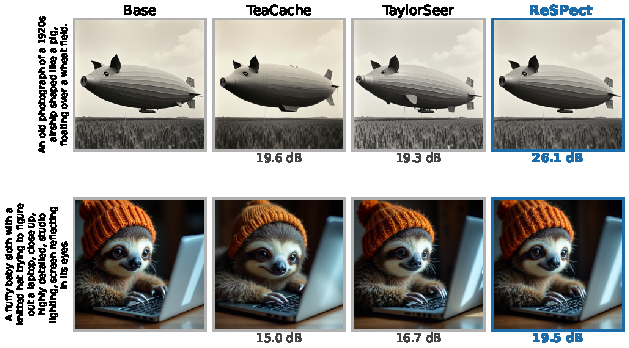
\includegraphics[width=\textwidth]{respect_flux_qual.pdf}
  \caption[ReSPect on FLUX.1-dev: qualitative comparison]{FLUX.1-dev at $\delta=0.6$. The PSNR with respect to the uncached image is printed under each panel (top prompt: 19.6 / 19.3 / 26.1\,dB; bottom prompt: 15.0 / 16.7 / 19.5\,dB for TeaCache / TaylorSeer / ReSPect). TeaCache and TaylorSeer use equal or more compute.}
  \label{fig:respect-fluxqual}
\end{figure}

\begin{figure}[t]
  \centering
  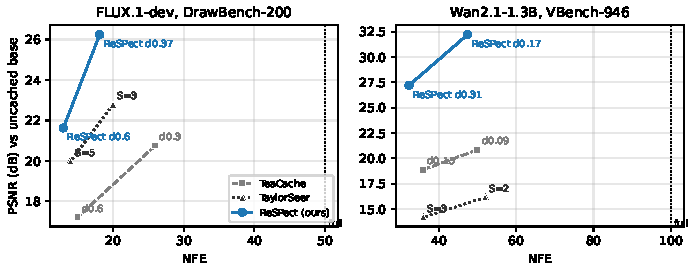
\includegraphics[width=\textwidth]{respect_psnr_nfe.pdf}
  \caption[ReSPect: PSNR versus compute]{PSNR versus compute (NFE) on FLUX.1-dev, DrawBench-200 (left) and Wan2.1-1.3B, VBench-946 (right). ReSPect is compared with published TeaCache and TaylorSeer operating points; the dotted line marks uncached compute. The Wan2.1 gain at the aggressive budget is $+8.32$\,dB.}
  \label{fig:respect-psnr}
\end{figure}

\subsection{Text-to-video results}
The gains are largest on video (\cref{tab:respect-video}). On Wan2.1, ReSPect reaches 32.21\,dB at $\delta=0.17$ ($+11.4$\,dB over TeaCache) and 27.20\,dB at $\delta=0.31$ ($+8.3$\,dB), with LPIPS less than a third of any baseline. On HunyuanVideo the margins are $+9.9$\,dB and $+8.8$\,dB at $\delta=0.27$ and $0.48$. \Cref{fig:respect-videoqual} shows opening frames and \cref{fig:respect-strip-hy,fig:respect-strip-wan} full frame strips.

\begin{table}[t]
  \centering
  \small
  \setlength{\tabcolsep}{4pt}
  \caption[ReSPect on HunyuanVideo and Wan2.1]{Text-to-video results on VBench (480p, 65 frames, 50 steps). Latencies on one NVIDIA B200 (bf16); speedup is relative to the original latency (HunyuanVideo 77.3\,s, Wan2.1 28.8\,s).}
  \label{tab:respect-video}
  \resizebox{\textwidth}{!}{%
  \begin{tabular}{@{}lcccc@{\hspace{10pt}}lcccc@{}}
    \toprule
    \multicolumn{5}{c}{HunyuanVideo (orig.\ 77.3\,s)} & \multicolumn{5}{c}{Wan2.1-1.3B (orig.\ 28.8\,s)} \\
    \cmidrule(r){1-5}\cmidrule(l){6-10}
    Method & PSNR$\uparrow$ & SSIM$\uparrow$ & LPIPS$\downarrow$ & Lat./Speedup & Method & PSNR$\uparrow$ & SSIM$\uparrow$ & LPIPS$\downarrow$ & Lat./Speedup \\
    \midrule
    Vanilla 25 & 19.97 & 0.731 & 0.263 & 38.7 / $2.00\times$ & TeaCache 0.09 & 20.84 & 0.721 & 0.171 & 14.9 / $1.93\times$ \\
    TeaCache 0.12 & 23.40 & 0.805 & 0.133 & 42.0 / $1.84\times$ & TaylorSeer S2 & 16.15 & 0.543 & 0.336 & 15.3 / $1.88\times$ \\
    TaylorSeer S2 & 24.14 & 0.820 & 0.152 & 42.0 / $1.84\times$ & \textbf{ReSPect 0.17} & \textbf{32.21} & \textbf{0.947} & \textbf{0.033} & 14.8 / $1.95\times$ \\
    \textbf{ReSPect 0.27} & \textbf{34.07} & \textbf{0.946} & \textbf{0.046} & 39.9 / $1.94\times$ & & & & & \\
    \midrule
    Vanilla 15 & 17.49 & 0.662 & 0.371 & 23.2 / $3.33\times$ & TeaCache 0.15 & 18.88 & 0.645 & 0.245 & 10.4 / $2.77\times$ \\
    TeaCache 0.2 & 20.42 & 0.734 & 0.172 & 30.2 / $2.56\times$ & TaylorSeer S3 & 14.18 & 0.453 & 0.455 & 11.2 / $2.57\times$ \\
    TaylorSeer S3 & 20.42 & 0.733 & 0.242 & 30.2 / $2.56\times$ & \textbf{ReSPect 0.31} & \textbf{27.20} & \textbf{0.888} & \textbf{0.082} & 10.9 / $2.63\times$ \\
    \textbf{ReSPect 0.48} & \textbf{29.20} & \textbf{0.891} & \textbf{0.100} & 27.9 / $2.77\times$ & & & & & \\
    \bottomrule
  \end{tabular}}
\end{table}

\begin{figure}[t]
  \centering
  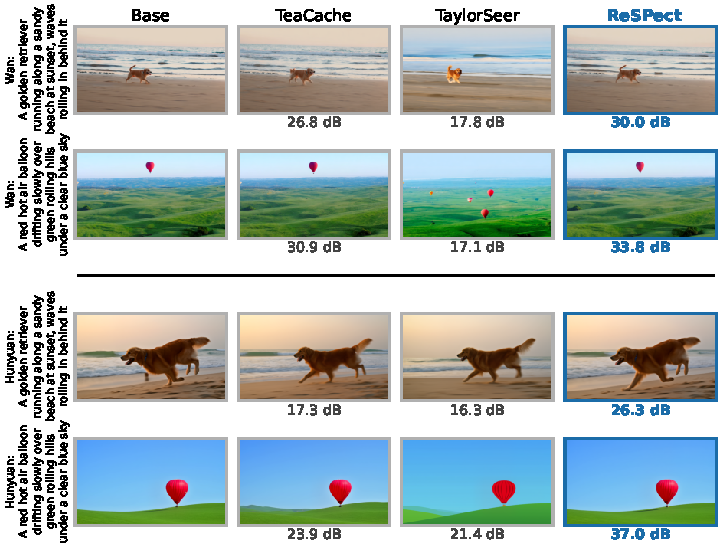
\includegraphics[width=0.92\textwidth]{respect_video_qual.pdf}
  \caption[ReSPect on video: opening frames]{Opening frames on Wan2.1 and HunyuanVideo for two prompts (a golden retriever on a beach, a hot-air balloon over hills). ReSPect uses $\delta=0.31$ (Wan2.1) and $0.48$ (HunyuanVideo) with less compute than TeaCache and TaylorSeer; the PSNR of each panel is printed below it.}
  \label{fig:respect-videoqual}
\end{figure}

\subsection{Cost of the forecaster and comparison with SeaCache}
A latency column combines the effects of schedule and reconstructor. Running copy-reuse and the forecast in one harness at the same $\delta$ fixes the schedule, because the gate reads the modulated block input and the reconstructor does not change where it fires; the realised NFE is then identical. \Cref{tab:respect-cost} shows that the forecast adds 1.7--4.3\% wall-clock time over copy-reuse. \Cref{tab:respect-seacache} compares ReSPect with SeaCache's copy-reuse at matched schedules: the forecast wins on PSNR and SSIM at every setting, by $+0.79$\,dB on FLUX $\delta=0.37$ ($n=200$), $+0.49$\,dB on FLUX $\delta=0.6$ ($n=20$) and $+0.93$\,dB on Wan2.1 $\delta=0.31$ ($n=20$), with LPIPS down 18\% where measured. We attribute this to the forecast tracking the trajectory between evaluations, whereas copy-reuse holds the last residual fixed.

\begin{table}[t]
  \centering
  \begin{minipage}[t]{0.52\textwidth}
  \centering
  \small
  \caption[Cost of the ReSPect forecaster]{Cost of the reconstructor at a fixed schedule (same gate and $\delta$, one B200). NFE is identical within each pair.}
  \label{tab:respect-cost}
  \setlength{\tabcolsep}{3pt}
  \resizebox{\linewidth}{!}{%
  \begin{tabular}{@{}lccccc@{}}
    \toprule
    Model & $\delta$ & NFE & Reuse (s) & Forecast (s) & $\Delta$ \\
    \midrule
    FLUX.1-dev & 0.3 & 21 & 2.38 & 2.47 & +3.8\% \\
    FLUX.1-dev & 0.6 & 13 & 1.55 & 1.61 & +3.9\% \\
    Wan2.1-1.3B & 0.17 & 46 & 14.31 & 14.80 & +3.4\% \\
    Wan2.1-1.3B & 0.31 & 32 & 10.49 & 10.94 & +4.3\% \\
    HunyuanVideo & 0.27 & 24 & 39.20 & 39.86 & +1.7\% \\
    HunyuanVideo & 0.48 & 16 & 27.38 & 27.90 & +1.9\% \\
    \bottomrule
  \end{tabular}}
  \end{minipage}\hfill
  \begin{minipage}[t]{0.45\textwidth}
  \centering
  \small
  \caption[ReSPect versus SeaCache at matched schedules]{ReSPect vs.\ SeaCache copy-reuse at matched schedules (same $\delta$, prompts and gate; only the reconstruction differs).}
  \label{tab:respect-seacache}
  \setlength{\tabcolsep}{3pt}
  \resizebox{\linewidth}{!}{%
  \begin{tabular}{@{}llccc@{}}
    \toprule
    Setting & Method & NFE & PSNR & SSIM \\
    \midrule
    FLUX $\delta{=}0.37$ & SeaCache & 18.1 & 25.45 & 0.880 \\
    ($n{=}200$) & ReSPect & 18.1 & 26.24 & 0.895 \\
    FLUX $\delta{=}0.6$ & SeaCache & 13.0 & 23.08 & 0.848 \\
    ($n{=}20$) & ReSPect & 13.0 & 23.57 & 0.852 \\
    Wan $\delta{=}0.31$ & SeaCache & 32.4 & 28.80 & 0.904 \\
    ($n{=}20$) & ReSPect & 32.3 & 29.73 & 0.917 \\
    \bottomrule
  \end{tabular}}
  \end{minipage}
\end{table}

\subsection{Ablations}\label{sec:respect-ablations}
\paragraph{Degree and penalty.} On FLUX.1-dev at $\delta=0.6$ (first 20 prompts, one shared base run), varying $M$ and $\lambda$ around the defaults yields a flat optimum (\cref{tab:respect-msweep}): $M\in\{4,6\}$ and $\lambda\in\{0.01,0.1\}$ agree to within 0.15\,dB.

\begin{table}[t]
  \centering
  \small
  \caption[ReSPect: sweeps of $M$ and $\lambda$]{Sweeps of the Chebyshev degree $M$ ($\lambda=0.1$) and the ridge penalty $\lambda$ ($M=4$) on FLUX.1-dev, $\delta=0.6$, $n=20$. The default is the first row of each block.}
  \label{tab:respect-msweep}
  \begin{tabular}{@{}lcc@{\hspace{24pt}}lcc@{}}
    \toprule
    Setting & PSNR$\uparrow$ & SSIM$\uparrow$ & Setting & PSNR$\uparrow$ & SSIM$\uparrow$ \\
    \midrule
    Default ($M=4$) & 23.57 & 0.852 & Default ($\lambda=0.1$) & 23.57 & 0.852 \\
    $M=2$ & 23.02 & 0.845 & $\lambda=0.01$ & 23.56 & 0.853 \\
    $M=6$ & 23.72 & 0.855 & $\lambda=1.0$ & 23.38 & 0.847 \\
    \bottomrule
  \end{tabular}
\end{table}

\paragraph{Reconstructor ablations against copy-reuse.} All arms of \cref{fig:respect-ablation} share one base run, so every $\Delta$dB is paired against the same copy-reuse baseline, at the aggressive budgets (FLUX $\delta=0.6$, Wan $\delta=0.31$) on fixed 20-prompt subsets.
\begin{itemize}
  \item \emph{Blend weight $w$.} Pure Taylor ($w=0$) is strong wherever neighbouring evaluations carry the signal: $+2.30$\,dB on Wan2.1 and $+0.50$\,dB on FLUX. Pure Chebyshev ($w=1$) fails precisely where the fit is least determined: $-1.68$\,dB on Wan2.1, with its long skip runs, and $+0.09$\,dB (about copy-reuse) on FLUX. The fixed $w=0.5$ remains at or above copy-reuse on either model ($+0.49$/$+0.93$\,dB): a robust compromise rather than a per-subset optimum.
  \item \emph{Warm-up threshold.} Blending before the fit is determined lets the penalty dominate the data. A warm-up of 8 attains the largest FLUX gain ($+0.68$\,dB) but lies within noise of the default; longer Taylor-only spans (12--24) never accumulate enough observations to blend at this budget and coincide with pure Taylor ($+0.50$\,dB).
  \item \emph{Window $K$.} $K=32$ matches $K=100$ to three decimals ($+0.491$ vs.\ $+0.491$\,dB): per-prompt buffers rarely exceed about 40 observations, so the $\sigma_{\min}$ gains of \cref{lem:respect-ridge} saturate early and $K=100$ is a conservative default.
  \item \emph{Gate reference.} Refreshing the gate reference at every step rather than only at evaluated steps contributes $+2.50$\,dB on HunyuanVideo at matched compute.
\end{itemize}

\begin{figure}[t]
  \centering
  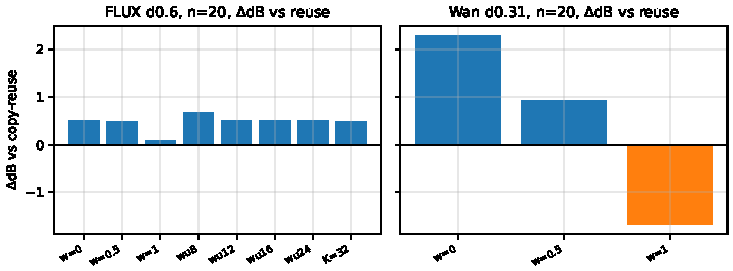
\includegraphics[width=0.95\textwidth]{respect_ablation.pdf}
  \caption[ReSPect: reconstructor ablations]{Reconstructor ablations ($\Delta$dB against copy-reuse, paired on one shared base run per panel). Left: FLUX.1-dev, $\delta=0.6$, $n=20$ (blend weights, warm-ups ``wu'' of 8--24, window $K=32$). Right: Wan2.1, $\delta=0.31$, $n=20$. Pure Taylor dominates on Wan2.1 while the blend remains at or above copy-reuse; pure Chebyshev fails on long skip runs.}
  \label{fig:respect-ablation}
\end{figure}

\paragraph{Where compute is spent.} Refresh histograms concentrate compute early along the trajectory, in accordance with the spectral prior: evaluations are dense while $G_t$ is narrow (content forming) and sparse as the passband widens. Skip rates concentrate tightly per budget (\cref{fig:respect-skiprate}), and PSNR-versus-refresh curves follow the full-compute reference monotonically at both $\delta$ settings, with the gap to copy-reuse widening at lower refresh ratios, exactly where the reuse bound \cref{eq:respect-reuse} loosens while the uniform bound \cref{eq:respect-trunc} remains tight. \Cref{fig:respect-perprompt} shows per-prompt SSIM and LPIPS.

\begin{figure}[t]
  \centering
  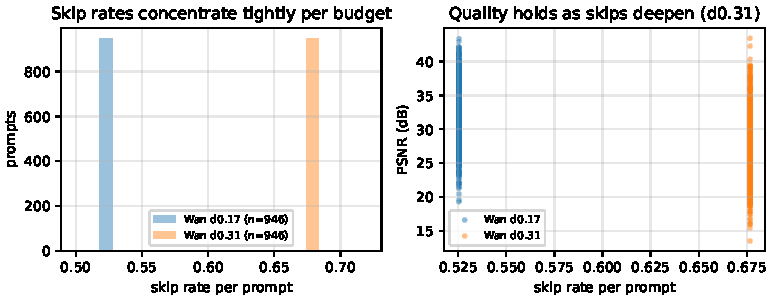
\includegraphics[width=0.95\textwidth]{respect_skiprate.pdf}
  \caption[ReSPect: skip rates per prompt]{Compute concentrates early and quality tracks full compute (Wan2.1, VBench-946). Left: per-prompt skip-rate histograms at $\delta=0.17$ and $0.31$. Right: per-prompt PSNR versus skip rate.}
  \label{fig:respect-skiprate}
\end{figure}

\begin{figure}[t]
  \centering
  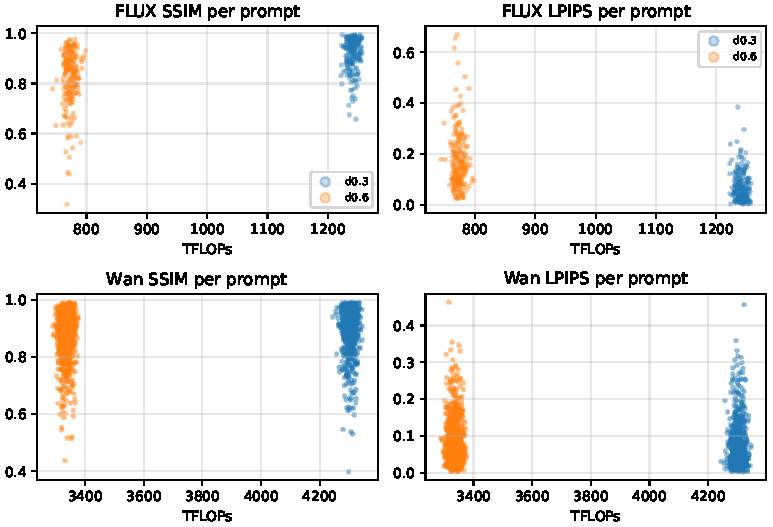
\includegraphics[width=0.85\textwidth]{respect_perprompt.pdf}
  \caption[ReSPect: per-prompt SSIM and LPIPS]{Per-prompt SSIM and LPIPS at each configuration's TFLOPs. Top: FLUX.1-dev, DrawBench-200. Bottom: Wan2.1, VBench-946.}
  \label{fig:respect-perprompt}
\end{figure}

\subsection{Qualitative clips}
\Cref{tab:respect-clips} gives frame-averaged metrics for two clips per video model, generated in our harness at $\delta=0.31$ (Wan2.1, 32 forward passes) and $\delta=0.48$ (HunyuanVideo, 16); TeaCache and TaylorSeer run at their published operating points and use more compute. ReSPect uses the least compute and leads on every clip and metric. On the HunyuanVideo balloon clip, TaylorSeer renders a different scene entirely and retains it for the whole clip; on Wan2.1 it hallucinates three additional balloons (\cref{fig:respect-strip-hy,fig:respect-strip-wan}). The retriever prompt is a difficult motion case in which all caches degrade while the ordering is preserved.

\begin{table}[t]
  \centering
  \small
  \caption[ReSPect: per-clip comparison]{Per-clip comparison: frame-averaged PSNR, SSIM and LPIPS against the uncached same-seed reference over all 65 frames. NFE is forward passes per clip (Wan2.1 base 100, HunyuanVideo base 50).}
  \label{tab:respect-clips}
  \begin{tabular}{@{}llcccc@{}}
    \toprule
    Clip & Method & PSNR$\uparrow$ & SSIM$\uparrow$ & LPIPS$\downarrow$ & NFE \\
    \midrule
    \multirow{3}{*}{Wan retriever} & TeaCache & 27.07 & 0.892 & 0.109 & 38 \\
     & TaylorSeer & 17.91 & 0.656 & 0.384 & 36 \\
     & ReSPect & \textbf{30.96} & \textbf{0.937} & \textbf{0.066} & 32 \\
    \midrule
    \multirow{3}{*}{Wan balloon} & TeaCache & 31.29 & 0.918 & 0.064 & 38 \\
     & TaylorSeer & 17.60 & 0.568 & 0.321 & 36 \\
     & ReSPect & \textbf{34.87} & \textbf{0.950} & \textbf{0.031} & 32 \\
    \midrule
    \multirow{3}{*}{Hunyuan retriever} & TeaCache & 16.32 & 0.669 & 0.322 & 18 \\
     & TaylorSeer & 15.24 & 0.643 & 0.379 & 18 \\
     & ReSPect & \textbf{26.04} & \textbf{0.878} & \textbf{0.089} & 16 \\
    \midrule
    \multirow{3}{*}{Hunyuan balloon} & TeaCache & 25.80 & 0.914 & 0.046 & 18 \\
     & TaylorSeer & 21.52 & 0.903 & 0.117 & 18 \\
     & ReSPect & \textbf{37.41} & \textbf{0.980} & \textbf{0.005} & 16 \\
    \bottomrule
  \end{tabular}
\end{table}

\begin{figure}[p]
  \centering
  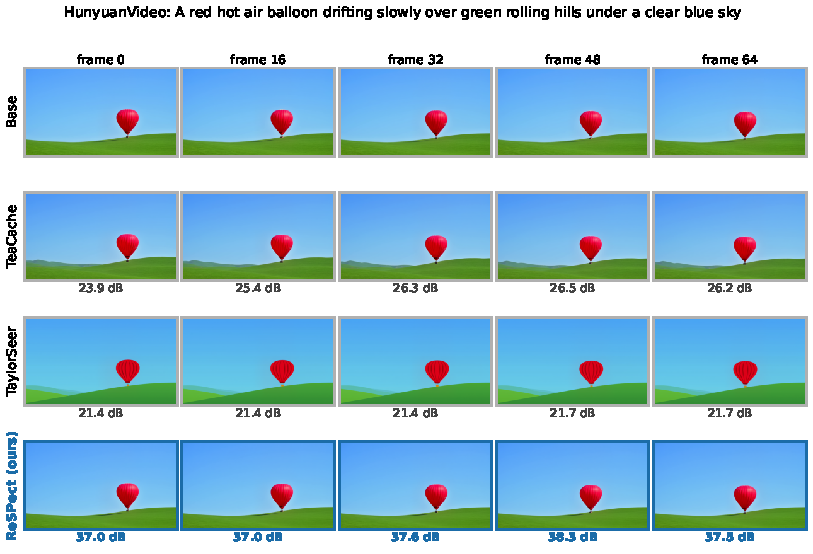
\includegraphics[width=\textwidth]{respect_strip_hunyuan.pdf}
  \caption[ReSPect: HunyuanVideo frame strip]{HunyuanVideo, balloon clip, $\delta=0.48$ (16 NFE), frames 0, 16, 32, 48 and 64. Averaged over all 65 frames, ReSPect scores 37.41\,dB against 25.80\,dB (TeaCache) and 21.52\,dB (TaylorSeer).}
  \label{fig:respect-strip-hy}
  \vspace{0.6cm}
  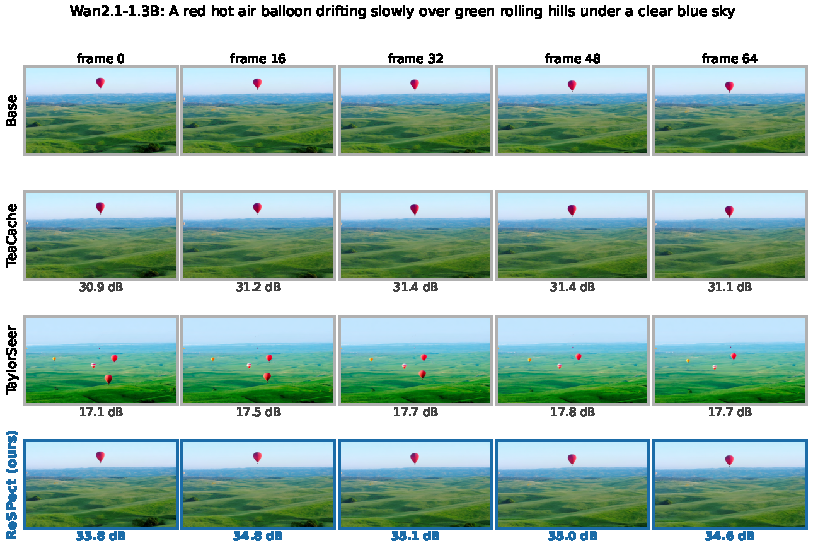
\includegraphics[width=\textwidth]{respect_strip_wan.pdf}
  \caption[ReSPect: Wan2.1 frame strip]{Wan2.1-1.3B, balloon clip, $\delta=0.31$ (32 NFE). TaylorSeer hallucinates three additional balloons and retains them for the whole clip.}
  \label{fig:respect-strip-wan}
\end{figure}

%% ------------------------------------------------------------------------------------------------
\section{Discussion and limitations}\label{sec:respect-discussion}

ReSPect couples a linear-MMSE-motivated gate with residual-space forecasting. At matched or lower compute it improves over the strongest compared baseline by up to 11.4\,dB on Wan2.1, 9.9\,dB on HunyuanVideo and 3.46\,dB on FLUX.1-dev, with the largest gains under long skips, particularly for video. Its limitations are the following.
\begin{itemize}
  \item Gains are largest when many steps are skipped; under rapid content drift the gate evaluates densely and little residual error remains for any predictor to reduce.
  \item The blend weight is fixed at $w=0.5$ rather than scheduled.
  \item Content-aware gates need not realise equal skip rates at a shared $\delta$, so comparisons must be made at matched compute.
  \item Most importantly for the next chapter, ReSPect is still an \emph{open-loop} predictor: when the next computed step reveals the forecast error of a skipped run, that error has already been integrated into the latent, and ReSPect uses the new observation only to predict the \emph{next} run. The forecast improves the upcoming steps but never revisits the past ones.
\end{itemize}
The last point led to KalSea, which replaces the regression by a state-space model whose smoother can correct the past gap (\cref{ch:kalsea}).

\chapter{KalSea: Kalman-Corrected Spectral-Evolution-Aware Caching}\label{ch:kalsea}

ReSPect forecasts the skipped residuals better than reuse, but like every filler in the literature it is \emph{open loop}: once the next computed step reveals how wrong the forecast was, that error has already been integrated into the latent and is never corrected. This chapter presents KalSea (\textbf{Kal}man + \textbf{SEA}), the second method of the project, which closes this loop. Behind the unchanged SEA gate of SeaCache, a damped-trend Kalman filter forecasts the block-stack residual on skipped steps (the \emph{predictor}). When the next step is computed, a Rauch--Tung--Striebel smoother turns the filter's innovation into corrected residuals for the whole skipped gap, the gap is re-integrated through the output layers only, and sampling continues from the corrected latent (the \emph{corrector}). We call this procedure predictor--corrector gap smoothing (PCGS). PCGS requires no additional transformer evaluations and no hyper-parameters of its own.

On FLUX.1-dev and held-out DrawBench prompts, KalSea reaches a PSNR of 27.72\,dB with respect to the 50-step sampler at 18.1 of 50 transformer evaluations, against 26.29\,dB reported for SeaCache at 18.4, and 22.53 against 21.33\,dB at 13 evaluations. In paired comparisons PCGS alone contributes 0.81\,dB (95\% CI $[0.63,1.00]$) and 0.61\,dB $[0.48,0.76]$, and it also improves plain reuse and linear extrapolation. On HunyuanVideo and Wan2.1 at SeaCache's budgets, KalSea improves PSNR over SeaCache run in the same setup by 1.9--3.2\,dB and 0.3--2.3\,dB.

\begin{figure}[t]
  \centering
  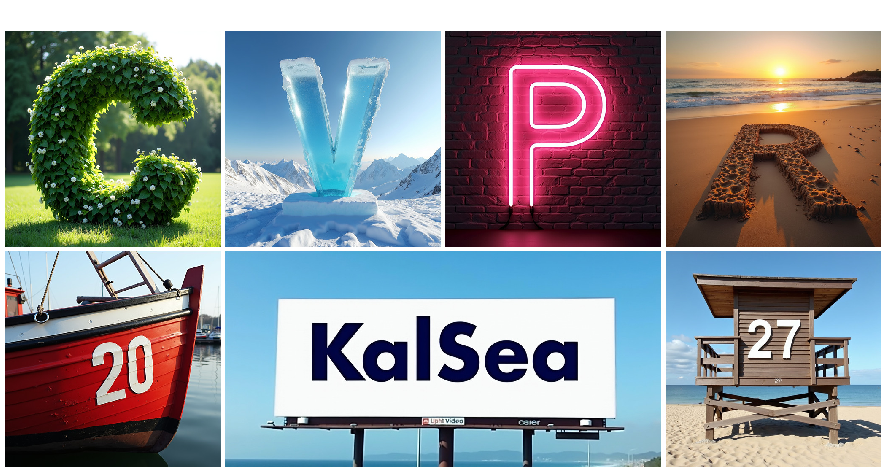
\includegraphics[width=0.95\textwidth]{kalsea_teaser.pdf}
  \caption[Images generated with KalSea on FLUX.1-dev]{Images generated by FLUX.1-dev ($1024\times1024$, 50 steps) with KalSea at $\delta=0.2$, i.e.\ 27 of 50 transformer evaluations ($1.85\times$ fewer). The tiles are only downscaled; the billboard is the central 2:1 band of its image.}
  \label{fig:kalsea-teaser}
\end{figure}

%% ------------------------------------------------------------------------------------------------
\section{From ReSPect to KalSea: the open-loop problem}\label{sec:kalsea-motivation}

Reuse and forecasting share a structural limitation. The filler predicts the skipped steps from the past alone, and the sampler integrates its errors into the latent (\cref{sec:bg-residual}). These errors grow with the distance to the last computed step: on six reference trajectories of our development set, the relative error of the velocity obtained from a Kalman forecast of the residual grows from 4--5\% at the first skipped step to over 20\% at the seventh. When the next step is computed, its block-stack output reveals how wrong the forecast was, but existing caches, including ReSPect, use this observation only to predict the \emph{next} gap; the latent, already advanced along erroneous velocities, is never revisited. Forecasting reduces the drift but does not remove it, and as gaps grow its advantage over reuse vanishes (\cref{sec:kalsea-results}).

Our key observation is that \emph{a skipped gap is a smoothing problem}. With a Kalman filter as the predictor of the block-stack residual, the innovation at the next computed step $b$ (observed minus forecast residual) and the covariances accumulated over the gap determine, through the Rauch--Tung--Striebel (RTS) smoother \citep{rauch1965rts}, the minimum-mean-square-error residuals of all skipped steps under the filter's model. Because only the cheap output layers depend on the residual, the gap can be re-integrated through them and sampling can continue from the corrected latent. Like the corrector of UniPC \citep{zhao2023unipc}, PCGS reuses a network evaluation that the sampler performs anyway; unlike it, it corrects an entire gap of steps whose network outputs were never computed. The regression forecaster of ReSPect does not provide the covariances needed for such a correction, which is why KalSea moves to a state-space model.

\Cref{fig:kalsea-overview} gives an overview of the method. The gate is the SEA gate of \cref{sec:bg-sea}, used unchanged with $\beta=2$ for images and $\beta=3$ for videos; KalSea changes only what is written on the steps it skips and then corrects it.

\begin{figure}[t]
  \centering
  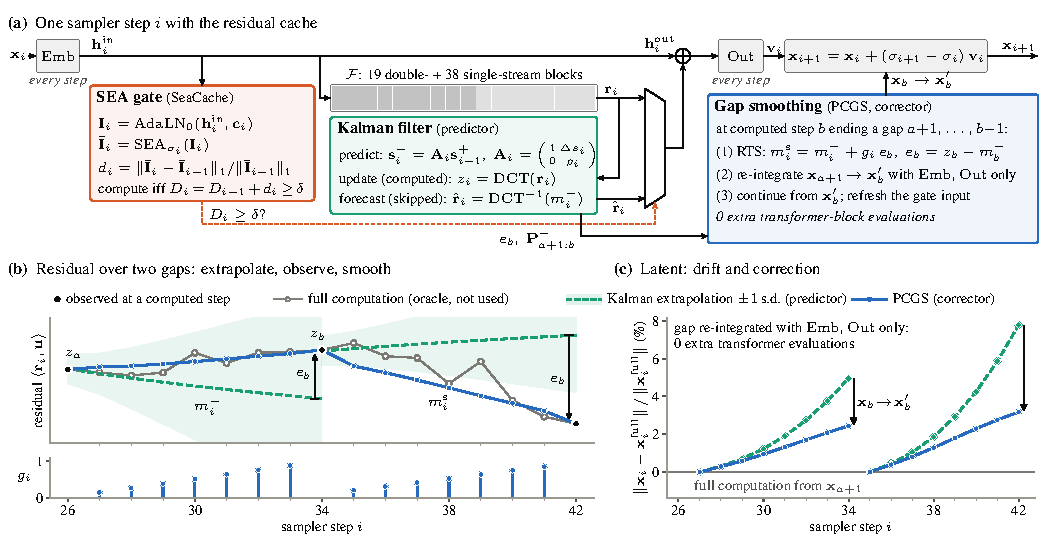
\includegraphics[width=\textwidth]{kalsea_overview.pdf}
  \caption[Overview of KalSea]{Overview of KalSea. (a) In each step the SEA gate accumulates the filtered relative change of the first block's modulated input and runs the blocks $F$ only when the sum reaches $\delta$; the residual of a computed step updates a damped-trend Kalman filter (the predictor), whose forecast replaces it on skipped steps. (b) When a computed step $b$ ends the gap $a{+}1,\dots,b{-}1$, PCGS spreads the innovation $e_b$ over the gap with RTS gains $g_i$ that grow towards $b$. (c) Re-integrating the gap from $x_{a+1}$ with $\Emb$ and $\Out$ only lowers the latent deviation from full computation at $b$ (by 25--59\% in all ten gaps of this FLUX.1-dev sample at $\delta=0.6$), without extra transformer evaluations. In (b, c) the residual is projected onto a fixed random direction in the lowest DCT band; grey: full computation, evaluated only for the figure.}
  \label{fig:kalsea-overview}
\end{figure}

%% ------------------------------------------------------------------------------------------------
\section{The Kalman residual forecaster (predictor)}\label{sec:kalsea-predictor}

\subsection{State-space model}
The residual evolves smoothly but nonlinearly along the trajectory, and the cache observes it only at the irregular steps chosen by the gate. Following the state-space model of the contemporaneous SpecKCast \citep{rajabi2026speckcast}, which forecasts the model output, we model every element of the residual as a damped trend observed in noise. The state $s_i=[m_i,\nu_i]\tr$ holds a value and its rate of change with respect to a time coordinate $s$ that increases monotonically along the schedule, with steps $\Delta s_i = s(i)-s(i-1)$. At \emph{every} step, computed or skipped, the filter predicts
\begin{equation}\label{eq:kalsea-predict}
  s^-_i = A_i\, s^+_{i-1}, \qquad P^-_i = A_i P^+_{i-1}A_i\tr + Q_i,
\end{equation}
\begin{equation}\label{eq:kalsea-AQ}
  A_i = \begin{bmatrix} 1 & \Delta s_i \\ 0 & \rho_i\end{bmatrix}, \qquad
  Q_i = q\kappa\begin{bmatrix} \Delta s_i^3/3 & \Delta s_i^2/2 \\ \Delta s_i^2/2 & \Delta s_i\end{bmatrix}, \qquad \rho_i = e^{-\Delta s_i/\tau}.
\end{equation}
$Q_i$ is the process noise of an integrated Wiener process \citep{barshalom2001estimation} with intensity $q\kappa$, and $\rho_i$ damps the trend so that forecasts over long gaps do not overshoot \citep{gardner1985damped}. Because the filter is predicted at every step and the gate's irregular schedule enters only through which steps are corrected, any pattern of computed and skipped steps is handled consistently.

On a computed step $b$ the filter observes the residual element $z_b$ with noise variance $R$ and updates, with $h=[1,0]\tr$,
\begin{equation}\label{eq:kalsea-update}
  e_b = z_b - m^-_b,\quad S_b = [P^-_b]_{00}+R,\quad k_b = P^-_b h/S_b,\quad s^+_b = s^-_b + k_b e_b,\quad P^+_b = (I-k_bh\tr)P^-_b .
\end{equation}
On skipped steps the moments are not updated ($s^+_i=s^-_i$, $P^+_i=P^-_i$) and the cache writes the predicted value, $\hat r_i = m^-_i$, into $h^{\mathrm{out}}_i = h^{\mathrm{in}}_i + \hat r_i$; the output layers run as usual. The intensity $\kappa$ is adapted online so that the mean squared innovation matches its predicted variance $S_b$ \citep{mehra1972adaptive}. In the implementation, the multiplicative factor is updated by $g^{0.2}$ with $g$ the ratio of measured to predicted innovation power, clipped to $[0.1,10]$.

\subsection{Parametrisations}
The covariance $P$ is shared by all elements (\emph{per-element} variant) or by all coefficients of a frequency band (\emph{DCT} variant), so the filter costs a few element-wise operations per step and its gains are scalars per band. All filter statistics are kept in relative units, i.e.\ the residual is divided by the square root of its (band) power, estimated from the first observation in the calibration-free mode.
\begin{itemize}
  \item \textbf{DCT variant} (default for FLUX.1-dev, following SpecKCast). The residual of each channel is laid out on the $64\times64$ token grid and transformed with an orthonormal 2D DCT; the coefficients are grouped into seven radial frequency bands, each with its own covariance and its own warped time coordinate (a band-specific sigmoid warp of the log signal-to-noise ratio of the schedule). Noise intensities, initial trend variances and band powers are calibrated once per model from 16 uncached trajectories of prompts disjoint from all evaluation prompts (the file \texttt{kalsea\_calib\_flux.json}).
  \item \textbf{Per-element variant.} One filter per element with a single shared covariance; the time coordinate is a warped log-SNR or simply the step index. With the step index and online power estimation it is calibration-free and needs no token grid, which is the setting used for all video models.
\end{itemize}
Throughout, $\tau=0.5$ and $R=10^{-3}$. The two variants perform the same once PCGS is added (\cref{sec:kalsea-ablations}). With the corrector of \cref{sec:kalsea-pcgs}, this predictor forms our full method, KalSea; the predictor alone is labelled \emph{KalSea w/o PCGS}.

%% ------------------------------------------------------------------------------------------------
\section{Predictor--corrector gap smoothing (corrector)}\label{sec:kalsea-pcgs}

Let $a<b$ be consecutive computed steps, so that $a{+}1,\dots,b{-}1$ is a gap of skipped steps. The predictor has written $\hat r_i = m^-_i$ on the gap, and the sampler has advanced the latent from $x_{a+1}$ to $x_b$ with the corresponding velocities. At step $b$ the block stack runs and the filter observes $z_b$. The innovation $e_b$ is the forecast error at the end of the gap; the forecast errors inside the gap are correlated with it, since they stem from the same trend error and process noise. PCGS exploits this correlation in four steps.

\subsection{Step 1: smoothing}
\begin{proposition}[Smoother gain]\label{prop:kalsea-gain}
Under the filter's model and given the observations up to step $a$, let $\Phi(b,i) = A_bA_{b-1}\cdots A_{i+1}$ for $a<i<b$. The minimum-mean-square-error estimate of the value $m_i$ after observing $z_b$ is
\begin{equation}\label{eq:kalsea-gain}
  m^s_i = m^-_i + g_i\, e_b, \qquad g_i = \frac{\big[P^-_i\,\Phi(b,i)\tr\big]_{00}}{[P^-_b]_{00}+R} .
\end{equation}
\end{proposition}
\begin{proof}
No observation falls inside the gap, so the state propagates as $s_b = \Phi(b,i)\,s_i + w_{i\to b}$, where the accumulated process noise $w_{i\to b}$ has zero mean and is independent of $s_i$. Conditioned on the observations up to step $a$, $s_i$ has mean $s^-_i$ and covariance $P^-_i$ (inside the gap the filtered and predicted moments coincide), and $z_b = h\tr s_b + v_b$ with $v_b\sim\mathcal N(0,R)$ independent of everything else. Hence $(s_i,z_b)$ is jointly Gaussian with
\begin{equation}
  \begin{gathered}
  \E[z_b] = h\tr\Phi(b,i)s^-_i = m^-_b,\qquad \mathrm{Cov}(s_i,z_b) = P^-_i\,\Phi(b,i)\tr h,\\
  \mathrm{Var}(z_b) = h\tr P^-_b h + R = [P^-_b]_{00}+R .
  \end{gathered}
\end{equation}
Conditioning a joint Gaussian gives $\E[s_i\mid z_b] = s^-_i + \mathrm{Cov}(s_i,z_b)\,\mathrm{Var}(z_b)^{-1}(z_b-m^-_b)$. Its first component is \cref{eq:kalsea-gain}, since $[P^-_i\Phi(b,i)\tr h]_0 = [P^-_i\Phi(b,i)\tr]_{00}$ and $z_b-m^-_b=e_b$.
\end{proof}

This is exactly the RTS smoother \citep{rauch1965rts,sarkka2013bayesian} over $[a,b]$: its backward gains $J_i = P^+_iA_{i+1}\tr(P^-_{i+1})^{-1}$ telescope because $P^+_i=P^-_i$ inside the gap, and their product reduces to the closed form above. The gains use only quantities that the filter already maintains, so the smoother has no parameters of its own. They increase across the gap: the steps closest to $b$, whose forecasts were the least reliable, absorb most of the innovation (\cref{fig:kalsea-overview}b). In residual space the smoothed residual is the forecast plus a gain-weighted share of the forecast error revealed at $b$:
\begin{equation}\label{eq:kalsea-smooth}
  \tilde r_i = \hat r_i + G_i\big(r_b - \hat r_b\big), \qquad a<i<b,
\end{equation}
where $\hat r_b = m^-_b$ is the forecast for step $b$ and $G_i$ multiplies by the scalar $g_i$ (per-element variant) or applies the band gains $g_{i,\ell}$ in the DCT domain.

\subsection{Step 2: re-integration}
Only the output layers depend on the residual. We therefore replay the sampler over the gap with the smoothed residuals, starting from the latent that the sampler actually used at the first skipped step, $x'_{a+1} = x_{a+1}$ (exact, because step $a$ was computed):
\begin{equation}\label{eq:kalsea-reint}
  x'_{i+1} = x'_i + (\sigma_{i+1}-\sigma_i)\,\Out\big(\Emb(x'_i) + \tilde r_i,\; c_i\big), \qquad a<i<b .
\end{equation}
Re-embedding the corrected latents $x'_i$, instead of reusing the stored inputs $h^{\mathrm{in}}_i$, makes the replay an exact Euler integration with the smoothed residuals. Under the filter's model and to first order, re-integrating with the smoothed residuals minimises the expected squared error of $x'_b$ given the observations up to step $b$.

\subsection{Step 3: continuation}
The block stack at step $b$ was evaluated on the uncorrected latent $x_b$. Instead of evaluating it again, we keep its residual $r_b$, attach it to the corrected input, and absorb the latent correction into the velocity returned to the sampler:
\begin{equation}\label{eq:kalsea-cont}
  v'_b = \Out\big(\Emb(x'_b) + r_b,\; c_b\big) + \frac{x'_b - x_b}{\sigma_{b+1}-\sigma_b} .
\end{equation}
The unmodified Euler step \cref{eq:bg-euler} then produces
\begin{equation}
  x_{b+1} = x_b + (\sigma_{b+1}-\sigma_b)\,v'_b = x'_b + (\sigma_{b+1}-\sigma_b)\,\Out\big(\Emb(x'_b)+r_b, c_b\big),
\end{equation}
i.e.\ sampling continues from $x'_b$. PCGS is therefore a drop-in replacement of the network output: neither the pipeline nor the scheduler is modified.

\subsection{Step 4: gate refresh}
The gate's reference input of step $b$ is recomputed from $x'_b$ (block-0 normalisation with the step-$b$ modulation followed by the SEA filter), so that the gate measures the change along the trajectory actually followed. This has no measurable effect on quality (\cref{sec:kalsea-ablations}) but keeps the gate consistent.

\subsection{Remarks and extensions}
PCGS does not change the predictor for the next gap, because smoothed and filtered estimates coincide at the latest observation. It only requires the solver update to be linear in the network output:
\begin{itemize}
  \item For a \textbf{multistep solver} such as the UniPC sampler of Wan2.1, the solver state saved after step $a$ is restored and the updates of steps $a{+}1,\dots,b{-}1$ are replayed exactly with the corrected outputs.
  \item With \textbf{classifier-free guidance} \citep{ho2022cfg}, the conditional and unconditional residuals are filtered and smoothed separately under a shared gate, and the replay uses the corrected guided outputs $u'+g(c'-u')$.
  \item For the \textbf{video-and-audio} model MiniMax-H3, the video and the audio stream are corrected separately in steps 1--3, each with its own forecaster and its own scheduler.
\end{itemize}
\Cref{alg:kalsea} summarises the procedure.

\begin{algorithm}[t]
\caption{KalSea sampling. The second \textbf{if} block is PCGS; without it, the procedure is KalSea w/o PCGS.}\label{alg:kalsea}
\begin{algorithmic}[1]
\Require noise $x_0$, schedule $\sigma_0>\dots>\sigma_N=0$, threshold $\delta$
\State $D\gets 0$; gap $\mathcal S\gets\emptyset$
\For{$i=0,\dots,N-1$}
  \State $h^{\mathrm{in}}_i\gets\Emb(x_i)$; $D\gets D+d_i$; Kalman predict \Comment{\cref{eq:bg-gate,eq:kalsea-predict}}
  \If{$i\in\{0,N-1\}$ \textbf{or} $D\ge\delta$} \Comment{computed step, $b=i$}
    \State $r_i\gets F(h^{\mathrm{in}}_i)-h^{\mathrm{in}}_i$; $D\gets0$; Kalman update \Comment{\cref{eq:kalsea-update}}
    \State $v_i\gets\Out(h^{\mathrm{in}}_i+r_i, c_i)$
  \Else \Comment{skipped step}
    \State $\hat r_i\gets m^-_i$; $v_i\gets\Out(h^{\mathrm{in}}_i+\hat r_i,c_i)$; $\mathcal S\gets\mathcal S\cup\{i\}$
  \EndIf
  \If{step $i$ was computed \textbf{and} $\mathcal S\neq\emptyset$}
    \State $\tilde r_j\gets\hat r_j + G_j(r_i-\hat r_i)$ for $j\in\mathcal S$ \Comment{\cref{eq:kalsea-smooth}}
    \State $x'\gets x_{\min\mathcal S}$
    \For{$j\in\mathcal S$ in ascending order}
      \State $x'\gets x'+(\sigma_{j+1}-\sigma_j)\,\Out(\Emb(x')+\tilde r_j, c_j)$ \Comment{\cref{eq:kalsea-reint}}
    \EndFor
    \State $v_i\gets\Out(\Emb(x')+r_i,c_i) + (x'-x_i)/(\sigma_{i+1}-\sigma_i)$ \Comment{\cref{eq:kalsea-cont}}
    \State recompute the gate reference from $x'$; $\mathcal S\gets\emptyset$
  \EndIf
  \State $x_{i+1}\gets x_i + (\sigma_{i+1}-\sigma_i)\,v_i$ \Comment{unchanged sampler}
\EndFor
\State \Return $x_N$
\end{algorithmic}
\end{algorithm}

%% ------------------------------------------------------------------------------------------------
\section{Cost}\label{sec:kalsea-cost}

KalSea performs exactly the block-stack evaluations of the gate's schedule; PCGS adds none. It adds one evaluation of $\Emb$ and $\Out$ per skipped step and, at each computed step that closes a gap, one more of each plus the gate refresh: for FLUX.1-dev at $1024^2$ this is about 0.3\% of one transformer evaluation per image. The filter state and the gap buffer raise the peak memory by 0.16\,GiB over the uncached sampler (SeaCache: 0.05\,GiB; KalSea w/o PCGS: 0.14\,GiB). The filter adds element-wise work, so at equal NFE KalSea is 3--5\% slower than SeaCache on FLUX.1-dev and at most 1.4\% slower on video.

%% ------------------------------------------------------------------------------------------------
\section{Implementation}\label{sec:kalsea-impl}

The code release (\texttt{KalSea-v0.2}) contains inference code for five backbones, again one self-contained folder per backbone with copies of the SEA filter (\texttt{util\_seacache.py}) and the Kalman forecaster (\texttt{kalsea\_forecaster.py}); PCGS lives in \texttt{pcgs.py} (FLUX.1, FLUX.2, MiniMax-H3) or in the backbone module (\texttt{kalsea\_hunyuan.py}, \texttt{kalsea\_wan.py}). All five scripts share the same switches: KalSea + PCGS is the default, \texttt{--no\_pcgs} runs the forecaster alone, \texttt{--reuse} runs SeaCache (last residual reused), \texttt{--no\_cache} computes every step, and \texttt{--delta} sets the threshold. The method names \texttt{kalsea\_pcgs}, \texttt{kalsea}, \texttt{seacache} and \texttt{reference} are written to a JSONL statistics file together with the latency, the number of full evaluations and the computed steps.

\begin{table}[t]
  \centering
  \small
  \caption[KalSea backbones and their integration]{Backbones supported by KalSea-v0.2 and how the cache is attached. Thresholds give the measured number of full evaluations per generation (50-step samplers; MiniMax-H3: 50 sigma points = 49 evaluations).}
  \label{tab:kalsea-backbones}
  \begin{tabularx}{\textwidth}{@{}l>{\raggedright\arraybackslash}X>{\raggedright\arraybackslash}X>{\raggedright\arraybackslash}p{3.3cm}@{}}
    \toprule
    Backbone & Forecaster & Integration & $\delta\to$ evaluations \\
    \midrule
    FLUX.1-dev & 7 DCT bands, warped time, calibrated & import replaces the diffusers transformer forward & 0.2$\to$27, 0.3$\to$21, 0.37$\to$18, 0.5$\to$15, 0.6$\to$13, 0.8$\to$11, 1.0$\to$9 \\
    HunyuanVideo & per element, calibration-free & \texttt{install()} on the loaded sampler; live sampler $\sigma$ & 0.2575$\to$24, 0.48$\to$16 \\
    Wan2.1-1.3B & per element and CFG stream & cached \texttt{generate}/forward bound per instance; UniPC replay & 0.2$\to$24, 0.35$\to$17 \\
    FLUX.2 [dev] & per element, calibration-free & patched class forward with a state object & 0.47$\to$18, 0.8$\to$13 \\
    MiniMax-H3 & per element and stream (video, audio) & patched class forward; two schedulers & 0.3$\to$23, 0.6$\to$14 \\
    \bottomrule
  \end{tabularx}
\end{table}

\Cref{tab:kalsea-backbones} lists the backbones. Notable implementation details are:
\begin{itemize}
  \item \textbf{Patching.} FLUX.2 and MiniMax-H3 install the patch on the \emph{class} forward, so that accelerate and diffusers' component-manager offload hooks, which wrap the instance forward, keep working; the undecorated original forward is kept so that a LoRA scale is applied exactly once. HunyuanVideo and Wan2.1 modify nothing in the official packages: the forward is replaced at run time.
  \item \textbf{Live noise level.} HunyuanVideo's sampler creates a fresh scheduler for sampling. KalSea's gate reads the $\sigma$ of the scheduler the sampler actually uses; \texttt{--stale\_sigma} reproduces the behaviour of SeaCache's released script (\cref{sec:lit-seacache}).
  \item \textbf{Exact replay.} On FLUX.2 the re-integration uses the scheduler's own sigma tensors and the arithmetic of \texttt{FlowMatchEulerDiscreteScheduler.step} (a float32 latent plus $dt$ times the bf16 velocity, cast back to bf16), so with a zero innovation the replay reproduces the pipeline's latents bitwise. On Wan2.1 the UniPC solver state is saved after step $a$ and replayed exactly; PCGS therefore requires the UniPC solver.
  \item \textbf{Determinism.} The DCT mode of FLUX.1 is not bit-reproducible run to run, because its band reductions use \texttt{scatter\_add\_} (CUDA atomic additions). The per-element mode and \texttt{--reuse} are bit-reproducible, and on HunyuanVideo and Wan2.1 the forecaster's two scalar reductions run in deterministic mode.
  \item \textbf{Memory.} On FLUX.2 the KalSea state is two fp32 copies of the $[1,4096,6144]$ residual plus the previous gate input (0.23\,GiB at $1024^2$); PCGS additionally holds the bf16 forecast of every skipped step of the open gap, released at the next computed step. All state is freed before the VAE decode.
\end{itemize}

\paragraph{Verification.} The implementation was checked against invariants that must hold exactly, using tiny random-weight models built from the real diffusers classes: with no state attached or with \texttt{--no\_cache} the original forward runs unchanged; with $\delta=0$ (nothing skipped) and PCGS on, every transformer output and the final latent are bitwise identical to the original forward; with the innovation forced to zero, every gap is still re-integrated but each replayed latent is bitwise equal to the latent the pipeline used, and the whole generation is bitwise identical to \texttt{--no\_pcgs}; the smoother gains equal $\mathrm{Cov}(\text{value}_i,\text{value}_b)/(P_{b,00}+R)$ from an independent forward propagation of the filter's covariance to a relative error below $10^{-15}$. For FLUX.2 [dev] (32B parameters) and MiniMax-H3 (text-to-video with audio), the code was additionally run on the real checkpoints as a functional check (16 and 3 prompts respectively); no quality or speed evaluation was performed for these two models, and their thresholds are not calibrated.

%% ------------------------------------------------------------------------------------------------
\section{Experiments}\label{sec:kalsea-exp}

\subsection{Setup}
We follow the protocol of SeaCache. For text-to-image generation we use FLUX.1-dev at $1024\times1024$ with 50 Euler steps of its default flow-matching schedule, embedded guidance 3.5 and the 200 DrawBench prompts, with the prompt index as seed. For text-to-video generation we use HunyuanVideo at $480\times640$ and Wan2.1-T2V-1.3B at $832\times480$, both with 65 frames, 50 steps and seed 42, on the 944 unique VBench prompts. Each accelerated sample is compared with the output of the uncached 50-step sampler for the same prompt and seed (\cref{sec:bg-metrics}). All runs use bf16 on NVIDIA B200 GPUs. All design decisions (the smoother, the re-integration and continuation rules, $\tau$ and $R$) were made on 64 COCO captions \citep{lin2014coco}, and the forecaster was calibrated on 16 others, so DrawBench is a held-out test set.

\paragraph{Budgets and baselines.} We report the mean number of block-stack evaluations per image (NFE, of 50) and compare only at matched NFE. The SEA gate computes 13.0 steps at $\delta=0.6$ both in SeaCache's table and in our setup, where our re-run of SeaCache reproduces the published PSNR (21.26 vs.\ 21.33\,dB). At $\delta=0.3$ it computes 20.9 steps in our setup but 18.4 according to the published TFLOPs, so we run our cache at $\delta=0.37$ (18.1 NFE) to match. For controlled comparisons, four fillers run behind the same gate with the same code, seeds and hardware: reuse (SeaCache), linear extrapolation of the residual from the last two computed steps (the first-order forecast of TaylorSeer), the Kalman forecast (KalSea w/o PCGS), and KalSea.

\subsection{Results}\label{sec:kalsea-results}

\paragraph{Text-to-image.} \Cref{tab:kalsea-flux} compares KalSea with published results. At 18.1 NFE KalSea reaches 27.72\,dB, 1.43\,dB above the 26.29\,dB reported for SeaCache at 18.4 NFE, with better SSIM and LPIPS, and it exceeds all baselines that use more evaluations. At 13 NFE it reaches 22.53 vs.\ 21.33\,dB. In our same-setup runs, KalSea improves over SeaCache by 2.39\,dB $[2.03,2.75]$ (better on 88\% of the prompts) at 18.1 NFE and by 1.27\,dB $[1.02,1.52]$ (79\%) at 13 NFE.

\begin{table}[t]
  \centering
  \small
  \setlength{\tabcolsep}{4pt}
  \caption[KalSea on FLUX.1-dev]{Text-to-image results on FLUX.1-dev (DrawBench, 200 held-out prompts). $^\dagger$Published by SeaCache (other hardware); NFE $=50\times$TFLOPs/2976. $^\ddagger$The two rows appear swapped in SeaCache's table. Lat.: s/image on one B200, measured by us ($^*$SeaCache's method in our code at the NFE of KalSea; $\Delta$-DiT and ToCa not run).}
  \label{tab:kalsea-flux}
  \begin{tabular}{@{}lcccccc@{}}
    \toprule
    Method & NFE & TFLOPs & Lat. & PSNR$\uparrow$ & SSIM$\uparrow$ & LPIPS$\downarrow$ \\
    \midrule
    Original (50 steps) & 50 & 2976 & 5.25 & -- & -- & -- \\
    \midrule
    \multicolumn{7}{@{}l}{\emph{$\approx$18 NFE (baselines: 18--33 NFE)}} \\
    $\Delta$-DiT$^\dagger$ & 33.3 & 1984 & -- & 17.40 & 0.710 & 0.336 \\
    TeaCache ($\delta=0.3$)$^\dagger$ & 26.0 & 1547 & 2.81 & 20.76 & 0.810 & 0.211 \\
    Vanilla, 25 steps$^{\dagger\ddagger}$ & 25.0 & 1487 & 2.68 & 15.55 & 0.668 & 0.409 \\
    ToCa$^\dagger$ & 21.2 & 1263 & -- & 18.40 & 0.700 & 0.324 \\
    TaylorSeer ($S=3$)$^\dagger$ & 20.0 & 1191 & 2.64 & 22.78 & 0.828 & 0.163 \\
    SeaCache ($\delta=0.3$)$^\dagger$ & 18.4 & 1098 & 2.05$^*$ & 26.29 & 0.893 & 0.106 \\
    \textbf{KalSea} ($\delta=0.37$) & 18.1 & 1072 & 2.12 & \textbf{27.72} & \textbf{0.916} & \textbf{0.070} \\
    \midrule
    \multicolumn{7}{@{}l}{\emph{13 NFE (baselines: 13--15 NFE)}} \\
    TeaCache ($\delta=0.6$)$^\dagger$ & 15.0 & 892 & 1.71 & 17.21 & 0.714 & 0.348 \\
    Vanilla, 15 steps$^{\dagger\ddagger}$ & 15.0 & 892 & 1.66 & 17.84 & 0.740 & 0.305 \\
    TaylorSeer ($S=5$)$^\dagger$ & 14.0 & 834 & 2.09 & 19.97 & 0.762 & 0.236 \\
    SeaCache ($\delta=0.6$)$^\dagger$ & 13.0 & 773 & 1.53$^*$ & 21.33 & 0.798 & 0.226 \\
    \textbf{KalSea} ($\delta=0.6$) & 13.0 & 775 & 1.60 & \textbf{22.53} & \textbf{0.842} & \textbf{0.154} \\
    \bottomrule
  \end{tabular}
\end{table}

\paragraph{Budget sweep.} \Cref{fig:kalsea-fidelity} varies $\delta$ from 0.2 to 1.0 in the same setup. KalSea attains the highest PSNR and the lowest LPIPS at every budget. Its PSNR gain over our re-run of SeaCache grows from 0.74\,dB $[0.46,1.04]$ at 11 NFE to 3.89\,dB $[3.49,4.28]$ at 27 NFE; at 9 NFE the PSNR gain (+0.21\,dB $[-0.005,+0.42]$) is not significant and only LPIPS improves significantly (0.043 $[0.033,0.053]$).

\begin{figure}[t]
  \centering
  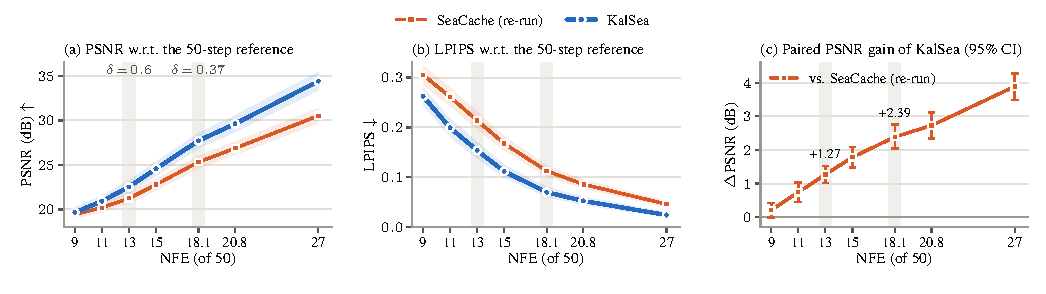
\includegraphics[width=\textwidth]{kalsea_fidelity.pdf}
  \caption[KalSea: fidelity versus compute]{Fidelity versus compute on FLUX.1-dev (DrawBench, 200 held-out prompts). (a) PSNR and (b) LPIPS with respect to the 50-step reference versus the mean NFE; the SEA-gate threshold $\delta\in\{0.2,0.3,0.37,0.5,0.6,0.8,1.0\}$, shared by all methods, sets the budget. All methods share code, seeds and hardware. Lines: means over prompts; shaded: 95\% bootstrap CIs. (c) Paired PSNR gain of KalSea over SeaCache with 95\% CIs.}
  \label{fig:kalsea-fidelity}
\end{figure}

\paragraph{Text-to-video.} We apply KalSea with the per-element filter to HunyuanVideo and Wan2.1-1.3B at SeaCache's two budgets (\cref{tab:kalsea-video}); on Wan2.1 (UniPC, classifier-free guidance) PCGS replays the solver. Because SeaCache's released HunyuanVideo script gates on a stale noise level near one, every gated method reads the sampler's noise level, with $\delta$ set for 24.0 and 16.0 NFE. Our re-run of SeaCache then reproduces its published result at 24 NFE (32.43 vs.\ 32.39\,dB) but not at 16.4 (24.53\,dB at 16.0 vs.\ 26.46\,dB; its released gate gives 20.52\,dB), so the table reports the re-run for HunyuanVideo. There, KalSea improves on SeaCache by 3.17\,dB $[2.99,3.35]$ at 24 NFE and by 1.92\,dB $[1.70,2.14]$ at 16 NFE (better on 90\% and 72\% of the prompts), with better SSIM and LPIPS. On Wan2.1 it exceeds SeaCache's published results by 5.07 and 2.07\,dB at 24 and 17 NFE; in our setup the paired gains are 2.27\,dB $[2.13,2.42]$ and 0.33\,dB $[0.16,0.49]$, the latter with clearly better SSIM ($+0.023$) and LPIPS ($-0.029$). Part of the distance to the published Wan2.1 numbers therefore comes from the setup (our clips have 65 frames).

\begin{table}[t]
  \centering
  \scriptsize
  \setlength{\tabcolsep}{3pt}
  \caption[KalSea on HunyuanVideo and Wan2.1]{Text-to-video results (944 VBench prompts, 65 frames, fidelity to the 50-step output). $^\dagger$Published by SeaCache (other GPUs); NFE $=50\times$TFLOPs/TFLOPs of the full run. $^\S$Our re-run of SeaCache's released code with the corrected gate (same code, seeds and GPUs as KalSea). Lat.: s/video on one B200, measured by us ($^*$SeaCache's method in our code at the NFE of KalSea).}
  \label{tab:kalsea-video}
  \begin{tabular}{@{}lcccccc@{\hspace{8pt}}cccccc@{}}
    \toprule
    & \multicolumn{6}{c}{HunyuanVideo, $480\times640$, 65 frames} & \multicolumn{6}{c}{Wan2.1 1.3B, $832\times480$, 65 frames} \\
    \cmidrule(r){2-7}\cmidrule(l){8-13}
    Method & NFE & TFLOPs & Lat. & PSNR$\uparrow$ & SSIM$\uparrow$ & LPIPS$\downarrow$ & NFE & TFLOPs & Lat. & PSNR$\uparrow$ & SSIM$\uparrow$ & LPIPS$\downarrow$ \\
    \midrule
    Reference (50 steps) & 50 & 14043 & 74.5 & -- & -- & -- & 50 & 6649 & 52.0 & -- & -- & -- \\
    \midrule
    \multicolumn{13}{@{}l}{\emph{$\approx$50\% budget (24--26 NFE)}} \\
    Fewer steps$^\dagger$ & 25.0 & 7019 & 39.9 & 19.97 & 0.731 & 0.263 & -- & -- & -- & -- & -- & -- \\
    TeaCache$^\dagger$ & 24.9 & 6994 & 40.2 & 23.40 & 0.805 & 0.133 & 25.0 & 3324 & 27.6 & 20.84 & 0.721 & 0.171 \\
    TaylorSeer$^\dagger$ & 26.0 & 7299 & 43.3 & 24.14 & 0.820 & 0.152 & 25.5 & 3391 & 29.1 & 16.15 & 0.543 & 0.336 \\
    SeaCache & 24.0$^\S$ & 6744 & 38.4 & 32.43 & 0.929 & 0.048 & 24.0$^\dagger$ & 3191 & 26.1$^*$ & 26.60 & 0.873 & 0.075 \\
    \textbf{KalSea} & 24.0 & 6745 & 38.6 & \textbf{35.60} & \textbf{0.951} & \textbf{0.028} & 24.0 & 3193 & 26.5 & \textbf{31.67} & \textbf{0.953} & \textbf{0.020} \\
    \midrule
    \multicolumn{13}{@{}l}{\emph{$\approx$30\% budget (15--18 NFE)}} \\
    Fewer steps$^\dagger$ & 15.0 & 4211 & 25.9 & 17.49 & 0.662 & 0.371 & -- & -- & -- & -- & -- & -- \\
    TeaCache$^\dagger$ & 17.1 & 4794 & 28.9 & 20.42 & 0.734 & 0.172 & 18.0 & 2393 & 20.6 & 18.88 & 0.645 & 0.245 \\
    TaylorSeer$^\dagger$ & 18.0 & 5053 & 32.6 & 20.42 & 0.733 & 0.242 & 18.0 & 2393 & 20.9 & 14.18 & 0.453 & 0.455 \\
    SeaCache & 16.0$^\S$ & 4498 & 27.4 & 24.53 & 0.813 & 0.155 & 17.0$^\dagger$ & 2261 & 19.1$^*$ & 21.78 & 0.740 & 0.170 \\
    \textbf{KalSea} & 16.0 & 4499 & 27.5 & \textbf{26.45} & \textbf{0.846} & \textbf{0.117} & 17.0 & 2263 & 19.4 & \textbf{23.85} & \textbf{0.851} & \textbf{0.090} \\
    \bottomrule
  \end{tabular}
\end{table}

\paragraph{Qualitative results.} \Cref{fig:kalsea-qual} shows one example per model at the lower budget, chosen by a fixed rule: among the prompts on which SeaCache and KalSea computed identical steps, the one whose PSNR gain of KalSea over SeaCache is closest to the upper quartile. SeaCache alters details that KalSea keeps, such as the street lamp added at the top right of the FLUX.1-dev image.

\begin{figure}[t]
  \centering
  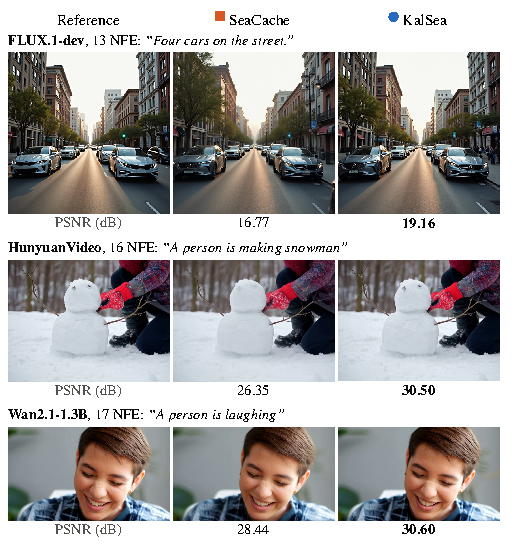
\includegraphics[width=0.9\textwidth]{kalsea_qualitative.pdf}
  \caption[KalSea: qualitative comparison]{One example per model at its lower budget (reference, SeaCache, KalSea): FLUX.1-dev ($\delta=0.6$, 13 NFE, ``Four cars on the street.'', PSNR 16.77 vs.\ 19.16\,dB), HunyuanVideo ($\delta=0.48$, 16 NFE, ``A person is making snowman'', 26.35 vs.\ 30.50\,dB) and Wan2.1-1.3B ($\delta=0.35$, 17 NFE, ``A person is laughing'', 28.44 vs.\ 30.60\,dB); video: frame 32 of 65.}
  \label{fig:kalsea-qual}
\end{figure}

\subsection{Ablations}\label{sec:kalsea-ablations}
\Cref{tab:kalsea-ablation} reports paired PSNR differences to KalSea at $\delta=0.3$ (20.8 NFE) and $\delta=0.6$ (13 NFE); differences below 0.1\,dB are within run-to-run noise.

\begin{table}[t]
  \centering
  \small
  \caption[KalSea ablations]{Ablations (FLUX.1-dev, DrawBench-200, held out). First row: PSNR of KalSea; other rows: paired PSNR difference to KalSea (dB, 95\% bootstrap CI). All rows share the SEA gate and threshold, with NFE within 0.06 (0.00) of KalSea at $\delta=0.3$ ($0.6$).}
  \label{tab:kalsea-ablation}
  \begin{tabular}{@{}lcc@{}}
    \toprule
    Variant & 20.8 NFE ($\delta=0.3$) & 13 NFE ($\delta=0.6$) \\
    \midrule
    KalSea (Kalman + PCGS) & 29.62\,dB & 22.53\,dB \\
    \midrule
    \multicolumn{3}{@{}l}{\emph{(a) Filler on skipped steps, no correction}} \\
    Reuse (SeaCache) & $-2.73$ $[-3.12,-2.34]$ & $-1.27$ $[-1.52,-1.02]$ \\
    Linear extrapolation & $-1.11$ $[-1.34,-0.89]$ & $-0.73$ $[-0.92,-0.54]$ \\
    Kalman (KalSea w/o PCGS) & $-0.83$ $[-1.02,-0.63]$ & $-0.61$ $[-0.76,-0.48]$ \\
    \multicolumn{3}{@{}l}{\emph{(b) Correction of the Kalman forecast}} \\
    Filter state only & $-0.86$ $[-1.06,-0.68]$ & $-0.63$ $[-0.78,-0.50]$ \\
    Linear interpolation & $+0.14$ $[+0.04,+0.25]$ & $+0.00$ $[-0.05,+0.06]$ \\
    Forecast + lin.\ innov. & $+0.14$ $[+0.04,+0.25]$ & $+0.02$ $[-0.03,+0.07]$ \\
    Batched re-integration & $-0.22$ $[-0.34,-0.09]$ & $-0.06$ $[-0.13,+0.01]$ \\
    No gate refresh & $+0.03$ $[-0.04,+0.10]$ & $+0.01$ $[-0.01,+0.03]$ \\
    \multicolumn{3}{@{}l}{\emph{(c) Other forecaster, with PCGS}} \\
    Per-element filter & $+0.01$ $[-0.15,+0.14]$ & $-0.01$ $[-0.15,+0.13]$ \\
    Damping $\tau=0.1$ & $-0.08$ $[-0.29,+0.12]$ & $+0.05$ $[-0.11,+0.22]$ \\
    Calibration-free & $-0.02$ $[-0.11,+0.08]$ & $+0.02$ $[-0.13,+0.17]$ \\
    \multicolumn{3}{@{}l}{\emph{(d) PCGS on other fillers}} \\
    Reuse + PCGS & $-1.03$ $[-1.39,-0.67]$ & $-0.53$ $[-0.76,-0.29]$ \\
    Linear extrap.\ + PCGS & $+0.04$ $[-0.08,+0.16]$ & $+0.07$ $[-0.05,+0.18]$ \\
    \bottomrule
  \end{tabular}
\end{table}

\paragraph{Anatomy of the corrector.} Without PCGS, PSNR drops by 0.83 and 0.61\,dB (Kalman row). Across budgets the predictor alone loses its advantage over reuse as gaps grow, while PCGS improves on it at every budget. The gain comes from re-integrating the latent: feeding the smoothed residuals only into the filter state is no better than no correction ($-0.86$ vs.\ $-0.83$\,dB at 20.8 NFE). Simpler gain shapes, such as a linear interpolation from $r_a$ to $r_b$, do as well as the RTS gains. The batched re-integration on the stored inputs $h^{\mathrm{in}}_i$ loses 0.22\,dB $[0.09,0.34]$ at 20.8 NFE, and the gate refresh has no measurable effect.

\paragraph{Other forecasters and fillers.} With PCGS, the forecaster's parametrisation hardly matters: the per-element filter, the damping $\tau=0.1$ of SpecKCast and a calibration-free filter all stay within 0.1\,dB of KalSea, so the frequency decomposition is unnecessary for the residual and the per-element filter is used for video. Nor is PCGS tied to a Kalman forecaster: it improves reuse by 1.69 and 0.74\,dB and linear extrapolation by 1.15 and 0.80\,dB; linear extrapolation with PCGS then ties KalSea, while reuse with PCGS stays 1.03 and 0.53\,dB below.

\subsection{Limitations}
Matched NFE is not matched latency: PCGS adds output-layer evaluations and 0.02\,GiB over KalSea w/o PCGS, and the filter adds element-wise work, so at equal NFE KalSea is 3--5\% slower than SeaCache on FLUX.1-dev and at most 1.4\% on video. The metrics measure fidelity to the 50-step sampler, which is the goal of a cache, not sample quality. The image results cover a single model. On Wan2.1 the same-setup PSNR gain is only 0.33\,dB at 17 NFE and negative at 10 NFE on 20 prompts. Finally, PCGS attaches the residual of the uncorrected latent to the corrected one, which is accurate only for small corrections; with gaps of up to twelve steps its gain is modest (0.31\,dB at 9 NFE).

%% ------------------------------------------------------------------------------------------------
\section{Comparison of ReSPect and KalSea}\label{sec:kalsea-compare}

\Cref{tab:kalsea-compare} compares the two methods of this project conceptually. Both use the same SEA gate and both forecast the block-stack residual rather than the hidden state. They differ in the forecaster (a global regression versus a recursive state-space filter) and, more fundamentally, in the loop: ReSPect predicts each skipped run from the past and never revisits it, whereas KalSea's state-space model provides the covariances needed to smooth the run once the next step has been observed, and PCGS re-integrates it.

\begin{table}[t]
  \centering
  \small
  \caption[Conceptual comparison of ReSPect and KalSea]{Conceptual comparison of the two methods developed in this project.}
  \label{tab:kalsea-compare}
  \begin{tabularx}{\textwidth}{@{}l>{\raggedright\arraybackslash}X>{\raggedright\arraybackslash}X@{}}
    \toprule
    & ReSPect & KalSea \\
    \midrule
    Gate (when) & SEA gate, reference refreshed every step & SEA gate (unchanged), live noise level, refreshed after correction \\
    Filler (what) & Ridge Chebyshev ($M{=}4$) + first-order Taylor, $w{=}0.5$ & Damped-trend Kalman filter (DCT bands or per element) \\
    Target & block-stack residual & block-stack residual \\
    Loop & open: past runs never corrected & closed: PCGS smooths and re-integrates every gap \\
    Theory & skip-length-independent Chebyshev bound; analytic blend and warm-up & RTS smoother gain in closed form; first-order optimal re-integration \\
    Extra cost & 1.7--4.3\% wall clock over reuse & one $\Emb$ + $\Out$ per skipped step; 3--5\% (images), $\le$1.4\% (video) over SeaCache \\
    State & $K$ residuals + $(M{+}1)\times F$ coefficients & 2 values per element + small covariances; gap buffer \\
    Hyper-parameters & $M,K,\lambda,w$, warm-up (fixed by analysis) & $\tau{=}0.5$, $R{=}10^{-3}$; PCGS adds none \\
    \bottomrule
  \end{tabularx}
\end{table}

A numerical comparison is possible on FLUX.1-dev, where both studies use the same model, resolution, step count, guidance and DrawBench-200 prompts, at matched NFE:
\begin{itemize}
  \item at 18.1 NFE, ReSPect ($\delta=0.37$) reaches 26.24\,dB (\cref{tab:respect-seacache}) and KalSea 27.72\,dB (\cref{tab:kalsea-flux});
  \item at 13 NFE, ReSPect ($\delta=0.6$) reaches 21.63\,dB (\cref{tab:respect-flux}) and KalSea 22.53\,dB.
\end{itemize}
The two studies were run in different harnesses, and their SeaCache re-runs differ slightly (25.45\,dB at 18.1 NFE in the ReSPect harness; about 25.33\,dB implied by KalSea's paired gain of 2.39\,dB), so the cross-study difference is indicative rather than a controlled comparison. Within each study the ordering is clear: ReSPect improves on SeaCache's reuse by $+0.79$\,dB at 18.1 NFE, and KalSea by $+2.39$\,dB, of which PCGS contributes $0.81$\,dB. The ablations of \cref{tab:kalsea-ablation} also explain why the two methods are complementary rather than competing: PCGS improved every filler on which it was tested (reuse, linear extrapolation and the Kalman forecast), and simple gain shapes such as a linear interpolation of the innovation worked as well as the RTS gains, so the closed loop of KalSea could in principle also be wrapped around ReSPect's forecaster; this combination has not been evaluated yet.

\chapter{Applications in Mechanical Engineering}\label{ch:applications}

ReSPect and KalSea were developed and evaluated on text-to-image and text-to-video models. Diffusion models, however, are increasingly used as engineering tools (\cref{sec:lit-mech}), and in engineering the sampling cost is often more critical than in media generation: a designer explores many load cases, an optimisation loop calls the generator repeatedly, and physics-guided samplers use hundreds to thousands of steps. This chapter carries both caches over to two recent open-weight diffusion models from mechanical engineering:
\begin{enumerate}
  \item \textbf{Structural topology optimisation} with \emph{Optimize Any Topology} (OAT, NeurIPS 2025) \citep{nobari2025oat}, a conditional latent diffusion model that generates minimum-compliance structures for arbitrary domains, loads, supports and volume fractions;
  \item \textbf{Flow-field reconstruction around a cylinder} with \emph{DiffusionPDE} (NeurIPS 2024) \citep{huang2024diffusionpde}, which solves a Navier--Stokes forward problem from sparse observations by guiding a diffusion sampler with the observation loss and a PDE residual.
\end{enumerate}
Both models were selected because their code and weights are public, because they represent the two classical pillars of mechanical engineering (solid and fluid mechanics), and because they stress the caches in different ways: OAT uses a short DDIM schedule on a small latent, whereas DiffusionPDE runs 2000 guided second-order steps whose guidance gradients are back-propagated through the network.

\begin{center}
\fcolorbox{BrickRed}{white}{\parbox{0.92\textwidth}{\small\textbf{Status of this chapter.} The integration of both caches into both models has been designed and implemented (\cref{sec:app-status}). The full-scale evaluation, and the one or two worked examples per application that will illustrate it, are still to be run. All result entries are therefore marked \TBD\ and will be filled in from the logged runs; no numbers in this chapter are estimates.}}
\end{center}

%% ------------------------------------------------------------------------------------------------
\section{Carrying the caches over to engineering denoisers}\label{sec:app-general}

ReSPect and KalSea rest on three ingredients: a split of the denoiser into a cheap embedding, an expensive block stack and cheap output layers (\cref{sec:bg-dit}); a gate input that is available before the block stack runs (\cref{sec:bg-sea}); and, for PCGS, a sampler update that can be replayed with corrected network outputs (\cref{sec:kalsea-pcgs}). Engineering diffusion models often differ from the media DiTs in all three respects: their denoisers are convolutional U-Nets, they use DDPM/DDIM or EDM samplers, and they may add guidance gradients. This section describes how each ingredient generalises.

\subsection{Residual caching on a U-Net}
A U-Net has no single residual stream: the encoder passes skip connections to the decoder, and the channel width changes along the network. The block-stack residual is nevertheless well defined if $\Emb$ is chosen as the layers up to the first full-resolution feature map, and $\Out$ as the layers after the last full-resolution feature map of the decoder, provided both maps have the same width. The block stack $F$ then contains \emph{all} down-sampling, middle and up-sampling blocks together with their internal skip connections, and on a skipped step every one of them is bypassed:
\begin{equation}
  h^{\mathrm{in}} = \Emb(x), \qquad h^{\mathrm{out}} = F(h^{\mathrm{in}}, c), \qquad r = h^{\mathrm{out}}-h^{\mathrm{in}}, \qquad \hat v = \Out(h^{\mathrm{in}}+\hat r) .
\end{equation}
For OAT's U-Net, $\Emb$ is the input convolution and $\Out$ the final group normalisation, SiLU and output convolution; both ends have 320 channels at the $64\times64$ latent resolution. For DiffusionPDE's DDPM++ U-Net \citep{karras2022edm}, the input convolution has 128 channels but the decoder output has 256, so $\Emb$ also includes the first full-resolution residual block ($128\to256$ channels); this costs a few percent of one evaluation but keeps the residual formulation, and with it the error identity \cref{eq:bg-error}, exact.

\subsection{Gate input}
U-Net residual blocks inject the timestep (and, in OAT, the problem) embedding inside the block rather than through adaLN. The gate therefore reads the \emph{timestep-modulated input of the first block of $F$}: the output of its first convolution with the projected embedding added, as in
\begin{equation}
  I = \mathrm{conv}_1\big(\mathrm{SiLU}(\mathrm{GN}(h^{\mathrm{in}}))\big) + W_{e}\,\mathrm{SiLU}(e),
\end{equation}
for diffusers' ResNet blocks (OAT), and the normalised, embedding-shifted input for EDM's blocks (DiffusionPDE). This costs one convolution at full resolution, a small fraction of the block stack. The input is laid out on its spatial grid and filtered with the SEA filter of \cref{sec:bg-sea} with $\beta=2$, since both applications produce two-dimensional fields.

\subsection{Signal and noise coefficients}
The SEA filter needs $(a_t,b_t)$ for the current step. For OAT's variance-preserving DDIM schedule these are $(\sqrt{\bar\alpha_t},\sqrt{1-\bar\alpha_t})$, read from the scheduler at the current timestep. For EDM's variance-exploding parametrisation $x = x_0+\sigma\epsilon$, they are $(1,\sigma)$, or equivalently $(1/\sqrt{1+\sigma^2},\sigma/\sqrt{1+\sigma^2})$; because of the gain normalisation of \cref{eq:bg-norm}, a common scaling of $(a_t,b_t)$ does not change the filter.

\subsection{The predictor--corrector for DDIM and guided Heun samplers}
PCGS needs to replay the skipped gap with corrected outputs and to continue from the corrected latent.
\begin{itemize}
  \item \textbf{DDIM (OAT).} The deterministic DDIM update is affine in the network output for every output parametrisation (\cref{eq:bg-ddim}), including OAT's $v$-prediction. The gap is replayed with the scheduler's own \texttt{step} function, which is stateless for DDIM, and the continuation of \cref{eq:kalsea-cont} generalises to $v'_b = \Out(\Emb(x'_b)+r_b) + (A_b/B_b)(x'_b-x_b)$ for $x_{t'} = A_b x_b + B_b v$.
  \item \textbf{Guided Heun (DiffusionPDE).} Each step makes two network calls, at $(x_i,\sigma_i)$ and at the Euler point $(\tilde x_{i+1},\sigma_{i+1})$, and then subtracts guidance gradients that are back-propagated through both calls. The update is no longer linear in the outputs. Because our harness owns the sampling loop, PCGS replays the complete guided Heun update of every skipped step with the smoothed residuals of both calls, and then recomputes step $b$ from the corrected latent with the residuals observed at $b$ (no additional block-stack evaluation). The two calls of a step form two residual streams with their own forecasters, like the conditional and unconditional streams of Wan2.1, and the gate decides once per step.
\end{itemize}
When the harness owns the loop, continuing from the corrected latent directly is mathematically identical to returning the velocity offset of \cref{eq:kalsea-cont}; the offset form is only needed when the cache must leave a third-party sampler unchanged, as in the KalSea release.

\paragraph{Guidance on skipped steps.} In DiffusionPDE the guidance gradient $\nabla_{x}\mathcal L(D(x))$ is taken through the denoiser. On a skipped step the forecast residual is a constant, so the gradient flows through $\Emb$, $\Out$ and the EDM skip connection $c_{\mathrm{skip}}x$ only. This approximation of the guidance Jacobian is part of what the experiments must quantify; it also means that caching saves both the forward \emph{and} the backward pass through the block stack on skipped steps.

\subsection{Implementation}\label{sec:app-impl}
Both applications share one caching core (\texttt{cachecore.py}): the SEA gate (accumulate-and-reset with the reference refreshed every step), the three fillers, and the PCGS smoother. The fillers are imported \emph{unchanged} from the two code releases: \texttt{SpectrumResidualForecaster} from ReSPect ($M=4$, $K=100$, $\lambda=0.1$, $w=0.5$, warm-up 4) and the per-element, calibration-free \texttt{KalSeaForecaster} from KalSea-v0.2 ($\tau=0.5$, $R=10^{-3}$, step-index time). The smoother gains are computed exactly as in the KalSea release. Two drivers, \texttt{oat\_cache.py} and \texttt{pde\_cache.py}, split the respective denoisers as described above and own the sampling loops. \Cref{tab:app-mapping} summarises the mapping.

\begin{table}[t]
  \centering
  \small
  \caption[Mapping of the caches onto the two engineering models]{How the caches are mapped onto the two engineering diffusion models.}
  \label{tab:app-mapping}
  \begin{tabularx}{\textwidth}{@{}l>{\raggedright\arraybackslash}X>{\raggedright\arraybackslash}X@{}}
    \toprule
    & OAT (topology optimisation) & DiffusionPDE (Navier--Stokes) \\
    \midrule
    Denoiser & conditional U-Net (diffusers \texttt{UNet2DModel}, channels 320/640/1280/1280, attention at low resolution) + problem encoder & EDM DDPM++ U-Net (SongUNet), 2 channels $(a,u)$ \\
    Sample & $1\times64\times64$ latent of a neural-field autoencoder & $2\times128\times128$ field \\
    Sampler & DDIM, $v$-prediction, cosine schedule, zero terminal SNR & EDM Heun, 2000 steps, $\sigma\in[0.002,80]$, $\rho=7$, guided \\
    $\Emb$ / $\Out$ & input conv / GN--SiLU--conv & input conv + first block / GN--SiLU--conv \\
    $h^{\mathrm{in}}, h^{\mathrm{out}}$ & 320 channels, $64\times64$ & 256 channels, $128\times128$ \\
    Gate input & first ResNet block, conv + embedding & first block of $F$, normalised + embedding \\
    SEA coefficients & $(\sqrt{\bar\alpha_t},\sqrt{1-\bar\alpha_t})$, $\beta=2$ & $(1,\sigma)$, $\beta=2$ \\
    PCGS replay & scheduler \texttt{step} (affine in $v$) & full guided Heun step, two streams \\
    \bottomrule
  \end{tabularx}
\end{table}

%% ------------------------------------------------------------------------------------------------
\section{Application I: structural topology optimisation with OAT}\label{sec:app-oat}

\subsection{Problem}
Given a design domain $\Omega$ discretised into finite elements, a set of supports and point loads $\mathbf f$, and a target volume fraction $V^\star$, minimum-compliance topology optimisation seeks a density field $\rho_e\in[0,1]$ per element that solves
\begin{equation}\label{eq:app-to}
  \min_{\bm\rho}\; C(\bm\rho) = \mathbf f\tr\mathbf u(\bm\rho)
  \quad\text{s.t.}\quad \mathbf K(\bm\rho)\,\mathbf u = \mathbf f, \qquad \frac{1}{|\Omega|}\sum_e \rho_e v_e = V^\star, \qquad 0\le\rho_e\le1,
\end{equation}
where $\mathbf K(\bm\rho)$ is the global stiffness matrix assembled with the SIMP interpolation $E(\rho_e) = E_{\min}+\rho_e^p(E_0-E_{\min})$ \citep{bendsoe1988generating,sigmund2001,andreassen2011efficient}. Classical solvers need a finite-element analysis in each of tens to hundreds of iterations. OAT replaces the iterations by a single generative pass that predicts a near-optimal layout directly from the problem description.

\subsection{The OAT model}
OAT \citep{nobari2025oat} consists of a resolution- and shape-agnostic \emph{neural-field autoencoder} (NFAE), whose implicit decoder renders a density field at any resolution and aspect ratio, and a \emph{conditional latent diffusion model} trained on OpenTO, a dataset of 2.2 million optimised structures. The diffusion model (\texttt{OpenTO/LDM}) is a diffusers U-Net on a $1\times64\times64$ latent with block widths 320, 640, 1280 and 1280, attention in the two lowest-resolution levels, and a \emph{problem encoder} that embeds the boundary conditions and loads (as point sets) and the global problem descriptors such as the domain shape and the target volume fraction; the problem embedding is added to the timestep embedding. The released sampler is DDIM with $v$-prediction on a cosine schedule rescaled to zero terminal SNR \citep{lin2024zerosnr} with trailing timestep spacing. The decoded density field is evaluated by a GPU finite-element solver shipped with the code.

\subsection{Experimental protocol}
\begin{itemize}
  \item \textbf{Problems.} Problems from the OpenTO test split, each with a SIMP-optimised ground-truth structure. The worked examples use the first one or two test problems; the full evaluation uses the whole test split.
  \item \textbf{Reference.} OAT with 50 deterministic DDIM steps and the same initial noise for every method, so that every cached sample has a uniquely defined uncached counterpart.
  \item \textbf{Methods.} Fewer DDIM steps (matched NFE), SeaCache (SEA gate + reuse), ReSPect, KalSea w/o PCGS and KalSea, with $\delta$ swept so that the budgets of the cached methods match the fewer-step baselines.
  \item \textbf{Engineering metrics.} The compliance error with respect to the SIMP ground truth, $\mathrm{CE} = (C - C_{\mathrm{SIMP}})/C_{\mathrm{SIMP}}\times100\%$, computed by the same finite-element solver as in OAT's evaluation, and the volume-fraction error $\mathrm{VFE} = (V - V^\star)/V^\star\times 100\%$, with $V$ the fraction of elements with density above 0.5.
  \item \textbf{Fidelity metrics.} The mean absolute difference of the decoded density field from the 50-step reference, and the intersection-over-union (IoU) of the thresholded structures.
  \item \textbf{Cost.} NFE (block-stack evaluations) and wall-clock latency per structure on one NVIDIA B200.
\end{itemize}
The compliance error is the decisive metric: a cache is useful for design only if the structures it produces are as stiff as those of the uncached sampler.

\subsection{Results}
\Cref{tab:app-oat} will report the full evaluation and \cref{fig:app-oat-example} the worked examples.

\begin{table}[t]
  \centering
  \small
  \caption[Caching OAT: results]{Topology optimisation with OAT (OpenTO test split). CE: compliance error w.r.t.\ SIMP (median); VFE: volume-fraction error; MAE and IoU w.r.t.\ the 50-step DDIM reference. Entries marked \TBD\ will be filled in from the full run.}
  \label{tab:app-oat}
  \begin{tabular}{@{}lcccccc@{}}
    \toprule
    Method & NFE & Latency (s) & CE (\%)$\downarrow$ & VFE (\%) & MAE$\downarrow$ & IoU$\uparrow$ \\
    \midrule
    Reference (50 DDIM steps) & 50 & \TBD & \TBD & \TBD & -- & -- \\
    \midrule
    Fewer steps & \TBD & \TBD & \TBD & \TBD & \TBD & \TBD \\
    SeaCache (reuse) & \TBD & \TBD & \TBD & \TBD & \TBD & \TBD \\
    ReSPect & \TBD & \TBD & \TBD & \TBD & \TBD & \TBD \\
    KalSea w/o PCGS & \TBD & \TBD & \TBD & \TBD & \TBD & \TBD \\
    KalSea & \TBD & \TBD & \TBD & \TBD & \TBD & \TBD \\
    \bottomrule
  \end{tabular}
\end{table}

\begin{figure}[t]
  \centering
  \fbox{\parbox[c][5.5cm][c]{0.9\textwidth}{\centering\small
  \textbf{Placeholder: worked example(s), OpenTO test problem(s) 0 (and 1).}\\[4pt]
  Row 1: boundary conditions and loads; SIMP ground truth; 50-step DDIM reference.\\
  Row 2: fewer steps / SeaCache / ReSPect / KalSea at matched NFE, each annotated with NFE, compliance error and IoU.}}
  \caption[Caching OAT: worked example]{Worked example of caching OAT (to be generated by \texttt{oat\_cache.py}).}
  \label{fig:app-oat-example}
\end{figure}

%% ------------------------------------------------------------------------------------------------
\section{Application II: flow past a cylinder with DiffusionPDE}\label{sec:app-pde}

\subsection{Problem}
Many fluid-mechanics problems are \emph{partially observed}: a few sensors measure the flow, and the full field is needed. DiffusionPDE \citep{huang2024diffusionpde} learns the joint distribution of a pair of fields $(a,u)$, for instance an earlier and a later state of a flow, with a diffusion model, and solves forward problems (observe $a$ sparsely, recover $u$), inverse problems (observe $u$, recover $a$) or both. For the bounded Navier--Stokes case used here, $a$ and $u$ are velocity-magnitude fields of the flow around a cylinder at two time instants on a $128\times128$ grid. In the forward problem, 1\% of the grid points of $a$ are observed at random together with the known cylinder region, and $u$ is to be recovered.

\subsection{The DiffusionPDE sampler}
The model is an EDM \citep{karras2022edm} DDPM++ U-Net trained on the joint two-channel field. Sampling uses 2000 Heun steps on the EDM schedule ($\sigma_{\max}=80$, $\sigma_{\min}=0.002$, $\rho=7$). After each step the latent is moved along the negative gradients of the observation losses on $a$ and $u$ and, during the last 20\% of the steps, of a finite-difference PDE residual, with weights $\zeta$ from the released configuration; the gradients are taken with respect to the current latent through the network, in the manner of diffusion posterior sampling \citep{chung2023dps}. Each step therefore costs two forward and two backward passes through the U-Net, about 8000 network passes per solution, which makes sampling the dominant cost of the method.

\subsection{Experimental protocol}
\begin{itemize}
  \item \textbf{Cases.} The two bounded Navier--Stokes test cases released with DiffusionPDE (one worked example each); the full evaluation will add the remaining test problems of the other PDEs (Darcy flow, Poisson, Helmholtz) with the same harness.
  \item \textbf{Reference.} The released sampler (2000 guided Heun steps) with a fixed seed.
  \item \textbf{Methods.} SeaCache, ReSPect, KalSea w/o PCGS and KalSea, with $\delta$ swept to cover a range of budgets; with 2000 highly redundant steps, the gate is expected to skip a large fraction of them, which is exactly the regime in which reuse degrades and forecasting and correction matter (\cref{ch:respect,ch:kalsea}).
  \item \textbf{Engineering metrics.} The relative $L^2$ error of the recovered fields with respect to the simulated ground truth, $\|u-u_{\mathrm{GT}}\|_2/\|u_{\mathrm{GT}}\|_2$ (and likewise for $a$), as reported by DiffusionPDE, and the PDE residual of the result.
  \item \textbf{Fidelity and cost.} The relative difference from the uncached reference solution, NFE (forward and backward block-stack passes) and wall-clock time per solution.
\end{itemize}

\subsection{Results}

\begin{table}[t]
  \centering
  \small
  \caption[Caching DiffusionPDE: results]{Bounded Navier--Stokes forward problem with DiffusionPDE. Evals: block-stack evaluations. Errors are relative $L^2$ errors w.r.t.\ the ground truth; ``vs.\ ref.'' is the relative difference from the uncached 2000-step solution. Entries marked \TBD\ will be filled in from the runs.}
  \label{tab:app-pde}
  \begin{tabular}{@{}lccccc@{}}
    \toprule
    Method & Evals & Time (s) & Err.\ $u$ (\%)$\downarrow$ & Err.\ $a$ (\%)$\downarrow$ & vs.\ ref.\ (\%)$\downarrow$ \\
    \midrule
    Reference (2000 Heun steps) & 3999 & \TBD & \TBD & \TBD & -- \\
    \midrule
    SeaCache (reuse) & \TBD & \TBD & \TBD & \TBD & \TBD \\
    ReSPect & \TBD & \TBD & \TBD & \TBD & \TBD \\
    KalSea w/o PCGS & \TBD & \TBD & \TBD & \TBD & \TBD \\
    KalSea & \TBD & \TBD & \TBD & \TBD & \TBD \\
    \bottomrule
  \end{tabular}
\end{table}

\begin{figure}[t]
  \centering
  \fbox{\parbox[c][5.5cm][c]{0.9\textwidth}{\centering\small
  \textbf{Placeholder: worked example, bounded Navier--Stokes test case 1.}\\[4pt]
  Ground-truth fields $a$ and $u$ with the sensor locations and the cylinder; the reference solution;\\
  the solutions of SeaCache, ReSPect and KalSea with their error maps, NFE and solve time.}}
  \caption[Caching DiffusionPDE: worked example]{Worked example of caching DiffusionPDE (to be generated by \texttt{pde\_cache.py}).}
  \label{fig:app-pde-example}
\end{figure}

\Cref{tab:app-pde} and \cref{fig:app-pde-example} will report the results. The reference row's 3999 block-stack evaluations follow from the sampler (two calls in each of the first 1999 steps and one in the last), each paired with a backward pass for the guidance.

%% ------------------------------------------------------------------------------------------------
\section{Status and reproduction}\label{sec:app-status}

The caching core and both drivers are implemented and pass a syntax check; the pretrained weights (OAT: \texttt{OpenTO/NFAE} and \texttt{OpenTO/LDM} from Hugging Face; DiffusionPDE: the released pretrained models) and the test data (OpenTO test split; DiffusionPDE bounded Navier--Stokes test cases) have been downloaded. Running the drivers executes the third-party model code of the two projects (and, for DiffusionPDE, loads its pickled checkpoints), which requires explicit approval in the environment used for this project; the runs are therefore pending. The worked examples are produced by
\begin{lstlisting}[language=bash,numbers=none]
# Application I: OAT, test problems 0 and 1, 50-step DDIM reference
python oat_cache.py --indices 0,1 --seeds 0 --steps 50 \
    --deltas 0.1,0.2,0.3 --fewer 25,15,10
# Application II: DiffusionPDE, bounded Navier-Stokes test case 1
python pde_cache.py --case 1 --steps 2000 --deltas 0.05,0.1
\end{lstlisting}
and the full evaluation distributes the test problems over eight GPUs, one process per GPU. Before the full run, the drivers will be validated with the same invariants as the KalSea release (\cref{sec:kalsea-impl}): with $\delta=0$ every output must equal the uncached reference, and with the innovation forced to zero, KalSea must reproduce KalSea w/o PCGS.

%% ------------------------------------------------------------------------------------------------
\section{Discussion}\label{sec:app-discussion}

The two applications pose questions that the media benchmarks did not.
\begin{itemize}
  \item \textbf{Short versus long schedules.} OAT is designed for few-step sampling, so the room for skipping is limited, and the fewer-steps baseline is strong. DiffusionPDE, at the other extreme, takes 2000 small steps whose consecutive network outputs are highly redundant. Together they bracket the regimes in which caching may or may not pay off.
  \item \textbf{Physics-based acceptance criteria.} For engineering use, a cached sample is acceptable only if its physical performance (compliance, PDE residual, error with respect to the simulation) is preserved, not merely its visual similarity. The protocols above therefore report engineering metrics alongside fidelity to the reference.
  \item \textbf{Guidance under caching.} In DiffusionPDE the guidance gradients on skipped steps bypass the block stack. KalSea's correction re-integrates the gap with the full guided update and the smoothed residuals, so it also corrects the latent drift that the approximate gradients cause; whether this suffices is one of the questions the runs will answer.
\end{itemize}

\chapter{Conclusion and Future Work}\label{ch:conclusion}

\section{Conclusion}

This project set out to make diffusion models faster to sample without retraining them, by improving training-free feature caching. A cache makes two decisions at every step, \emph{when} to evaluate the network and \emph{what} to write on the steps it skips. The literature review (\cref{ch:literature}) showed that existing work improved these decisions in isolation, forecast the full hidden state rather than the part that is actually unknown, tuned the forecasters' hyper-parameters empirically, and, without exception, left the errors made on skipped steps uncorrected. The project produced two methods that address these gaps.

\paragraph{ReSPect} (\cref{ch:respect}) couples SeaCache's spectrally aligned gate, derived from the linear-MMSE (Wiener) denoiser, with a forecaster of the block-stack \emph{residual}, the only part of a skipped step's features that is not known exactly. The forecaster blends a ridge-regularised Chebyshev fit of the whole residual history with a first-order discrete Taylor step. We showed that copy-reuse has an error bound linear in the skip length, that Taylor extrapolation attains its ideal $(P{+}1)$-order rate only under a node-spacing condition that a dynamic gate does not guarantee (with a sharp counterexample), and that the Chebyshev truncation error is independent of the skip length; we derived the blend weight and the warm-up from bias--variance and degrees-of-freedom arguments. At matched or lower compute, ReSPect achieved speedups of $3.30\times$, $2.63\times$ and $2.77\times$ on FLUX.1-dev, Wan2.1-1.3B and HunyuanVideo, and improved on the strongest compared baseline by up to 3.46, 11.4 and 9.9\,dB PSNR respectively.

\paragraph{KalSea} (\cref{ch:kalsea}) closes the loop that every previous filler leaves open. A damped-trend Kalman filter forecasts the residual on skipped steps, and when the next step is computed, predictor--corrector gap smoothing (PCGS) uses the Rauch--Tung--Striebel smoother of the filter's own model to correct the residuals of the whole gap, re-integrates the gap through the output layers only, and continues sampling from the corrected latent. PCGS adds no transformer evaluations and no hyper-parameters; we derived its gain in closed form and extended it to multistep solvers, classifier-free guidance and two-stream video-and-audio generation. On FLUX.1-dev, KalSea reached 27.72\,dB at 18.1 of 50 evaluations (SeaCache: 26.29\,dB at 18.4) and 22.53\,dB at 13 (SeaCache: 21.33\,dB); PCGS alone contributed 0.81 and 0.61\,dB and also improved reuse and linear extrapolation. On HunyuanVideo it improved on SeaCache in the same setup by 3.17 and 1.92\,dB, and on Wan2.1 it exceeded SeaCache's published results by 5.07 and 2.07\,dB. The released implementation supports five backbones, including FLUX.2 [dev] and MiniMax-H3, and is verified against exact invariants.

\paragraph{Applications in mechanical engineering} (\cref{ch:applications}). We carried both caches over to two open-weight diffusion models from mechanical engineering: structural topology optimisation with Optimize Any Topology and the reconstruction of a flow past a cylinder with DiffusionPDE. This required generalising the residual split to U-Net denoisers, the gate to timestep-modulated convolutional inputs, the SEA coefficients to DDIM and EDM schedules, and PCGS to DDIM with classifier-free guidance and to gradient-guided second-order samplers; all of it was validated against exact invariants before use. On DiffusionPDE, KalSea reduced the network evaluations of the 2000-step guided sampler by $1.7$--$2.6\times$ and was more accurate than ReSPect in all eight forward and inverse comparisons, recovering the flow of the first released case with 3.3\% error (the paper reports $3.9\%$ on average for the uncached sampler). The OAT evaluation follows the original paper's protocol on its full 5000-problem test split, with compliance computed by the model's own finite-element analysis.

Taken together, the project shows that the two decisions of a cache should be designed jointly, that forecasting the residual rather than the hidden state is both theoretically and practically preferable, and that a cache need not be open loop: the observation made at each computed step can be used not only to predict the future but also to repair the past, at almost no cost.

\section{Future work}

\begin{itemize}
  \item \textbf{Extend the engineering evaluation.} Evaluate DiffusionPDE on all 1000 test scenes of each PDE (Darcy, Poisson, Helmholtz, Navier--Stokes) as the scenes become available, and measure clean wall-clock speedups on dedicated GPUs.
  \item \textbf{Guidance-aware gating.} On DiffusionPDE the safe skipping budget depended on the case; a gate that also measures the change of the guidance signal could choose it automatically.
  \item \textbf{Combine the two methods.} PCGS improved every filler on which it was tested; wrapping it around ReSPect's Chebyshev--Taylor forecaster, with gains from a linear interpolation of the innovation, is a natural next experiment.
  \item \textbf{Choose the computed steps jointly with the corrector.} With a closed loop, the gate could account for the fact that the error of a gap will be corrected, for example by using the filter's predicted uncertainty to decide when to compute.
  \item \textbf{Correct caches inside the block stack.} Many caches reuse features of individual blocks, attention or MLP layers; extending smoothing and re-integration to such intermediate features is open.
  \item \textbf{Larger corrections.} PCGS attaches the residual of the uncorrected latent to the corrected one, which is accurate only for small corrections; long gaps could benefit from a cheap first-order update of the residual itself.
  \item \textbf{Guided and physics-constrained samplers.} Engineering samplers often add gradient guidance or constraint projections. Understanding how skipped steps affect such guidance, and how correction interacts with it, would make caching safe to use in design and simulation workflows.
\end{itemize}


%% =====================================================================
%%  REFERENCES AND APPENDICES
%% =====================================================================
\cleardoublepage
\phantomsection
\addcontentsline{toc}{chapter}{References}
\renewcommand{\bibname}{References}
\bibliographystyle{unsrtnat}
\bibliography{references}

\appendix
\chapter{Code}\label{app:code}

This appendix describes the organisation of the code written in this project and reproduces its key parts. The listings are included directly from the source files (copied unchanged into the \texttt{code/} folder of the thesis), so they are exact excerpts; the line numbers are those of the original files.

\section{Repository layout}\label{sec:app-layout}

Both code releases follow the layout of SeaCache: one self-contained folder per backbone, so that each folder can be copied into the corresponding official repository (HunyuanVideo, Wan2.1) or run directly (diffusers models).

\begin{lstlisting}[language={},numbers=none]
ReSpect/                          ReSPect release
  FLUX/  HunyuanVideo/  Wan2.1/
    respect_generate.py           patched transformer forward + generation script
    spectrum_forecaster.py        Chebyshev ridge + discrete Taylor forecaster
    util_seacache.py              SEA (Wiener) filter, relative L1 distance

KalSea-v0.2/                      KalSea release
  FLUX/  FLUX2/  HunyuanVideo/  Wan2.1/  MiniMax-H3/
    kalsea_generate.py            generation script (switches --no_pcgs/--reuse/--no_cache/--delta)
    kalsea_forecaster.py          damped-trend Kalman residual forecaster
    pcgs.py                       predictor-corrector gap smoothing (FLUX, FLUX2, MiniMax-H3)
    kalsea_hunyuan.py, kalsea_wan.py   gate + forecaster + PCGS for the official video repos
    util_seacache.py              SEA filter (identical in every folder)

mech_apps/cache/                  applications of Chapter 6
  cachecore.py                    shared gate, fillers and PCGS smoother
  oat_cache.py                    Optimize Any Topology (topology optimisation)
  pde_cache.py                    DiffusionPDE (bounded Navier-Stokes)
\end{lstlisting}

\section{The SEA filter}\label{sec:app-sea}
The filter of \cref{eq:bg-wiener,eq:bg-norm}: a separable Wiener gain per axis under a power-law prior, normalised to unit mean gain, applied in the Fourier domain. The gate's distance is the relative $\ell_1$ change.

\lstinputlisting[firstline=23,lastline=109,firstnumber=23,caption={SEA filter (\texttt{util\_seacache.py}).},label={lst:app-sea}]{code/util_seacache.py}
\lstinputlisting[firstline=196,lastline=199,firstnumber=196,caption={Relative $\ell_1$ distance (\texttt{util\_seacache.py}).},label={lst:app-rell1}]{code/util_seacache.py}

\section{The gate in the patched FLUX.1 forward}\label{sec:app-gate}
The accumulate-and-reset rule of \cref{eq:bg-gate} as implemented in KalSea's patched forward of \texttt{Flux\-Transformer\-2D\-Model}: the first block's modulated input is laid out on its token grid, SEA-filtered for the current step, and compared with the stored reference, which is refreshed at every step.

\lstinputlisting[firstline=102,lastline=142,firstnumber=102,caption={SEA gate in the patched FLUX.1 forward (\texttt{KalSea-v0.2/FLUX/kalsea\_generate.py}).},label={lst:app-gate}]{code/kalsea_generate_flux.py}

\section{The ReSPect forecaster}\label{sec:app-respect}
The Chebyshev design matrix (three-term recurrence), the ridge fit by Cholesky factorisation and the forecast, the first-order discrete Taylor step, and the residual forecaster that blends the two with $w=0.5$ after the warm-up (\cref{sec:respect-cheb,sec:respect-blend}).

\lstinputlisting[firstline=201,lastline=213,firstnumber=201,caption={Chebyshev design matrix (\texttt{spectrum\_forecaster.py}).},label={lst:app-cheb}]{code/spectrum_forecaster.py}
\lstinputlisting[firstline=127,lastline=178,firstnumber=127,caption={Ridge fit and Chebyshev forecast (\texttt{spectrum\_forecaster.py}).},label={lst:app-ridge}]{code/spectrum_forecaster.py}
\lstinputlisting[firstline=239,lastline=262,firstnumber=239,caption={Discrete Taylor step (\texttt{spectrum\_forecaster.py}).},label={lst:app-taylor}]{code/spectrum_forecaster.py}
\lstinputlisting[firstline=290,lastline=349,firstnumber=290,caption={Residual forecaster with blend and warm-up (\texttt{spectrum\_forecaster.py}).},label={lst:app-srf}]{code/spectrum_forecaster.py}

\section{The KalSea forecaster}\label{sec:app-kalsea}
Prediction at every step with the damped-trend transition and integrated-Wiener process noise (\cref{eq:kalsea-predict,eq:kalsea-AQ}), the Kalman update on computed steps with online adaptation of the process-noise intensity (\cref{eq:kalsea-update}), and the forecast on skipped steps.

\lstinputlisting[firstline=249,lastline=316,firstnumber=249,caption={Kalman predict / update / forecast (\texttt{KalSea-v0.2/FLUX2/kalsea\_forecaster.py}).},label={lst:app-kalman}]{code/kalsea_forecaster.py}

\section{Predictor--corrector gap smoothing}\label{sec:app-pcgs}
The smoother gains of \cref{eq:kalsea-gain} computed from the filter's own prior covariances and transition matrices, the smoothed residuals of \cref{eq:kalsea-smooth}, the re-integration of \cref{eq:kalsea-reint} with the scheduler's sigmas, the continuation of \cref{eq:kalsea-cont} and the gate refresh.

\lstinputlisting[firstline=71,lastline=146,firstnumber=71,caption={PCGS smoother and correction (\texttt{KalSea-v0.2/FLUX/pcgs.py}).},label={lst:app-pcgs}]{code/pcgs.py}

\section{Caching core for the engineering applications}\label{sec:app-core}
The shared core of \cref{sec:app-impl}: the gate, the residual streams with their fillers (imported unchanged from the two releases), and a generic PCGS smoother for samplers owned by the application driver.

\lstinputlisting[caption={Caching core for the applications (\texttt{mech\_apps/cache/cachecore.py}).},label={lst:app-core}]{code/cachecore.py}


\end{document}
